\documentclass{article}
% if you need to pass options to natbib, use, e.g.:
\PassOptionsToPackage{}{natbib}
% before loading neurips_2024


% ready for submission
% \usepackage{neurips_2024}


% to compile a preprint version, e.g., for submission to arXiv, add add the
% [preprint] option:
%     \usepackage[preprint]{neurips_2024}

% to compile a camera-ready version, add the [final] option, e.g.:
\usepackage[final]{neurips_2024}

% to avoid loading the natbib package, add option nonatbib:
%    \usepackage[nonatbib]{neurips_2024}


% ============================================================
\usepackage[utf8]{inputenc} % allow utf-8 input
\usepackage[T1]{fontenc}    % use 8-bit T1 fonts
%\usepackage{hyperref}       % hyperlinks
\usepackage{url}            % simple URL typesetting
\usepackage{booktabs}       % professional-quality tables
\usepackage{amsfonts}       % blackboard math symbols
\usepackage{nicefrac}       % compact symbols for 1/2, etc.
\usepackage{microtype}      % microtypography
\usepackage{xcolor}         % colors
\usepackage[colorlinks=true,
            linkcolor=red,
            citecolor=blue,
            filecolor=blue,
            urlcolor=blue]{hyperref}
%============================================================
\usepackage{amsmath}
\allowdisplaybreaks[4]
\usepackage{ntheorem}
\newtheorem{theorem}{Theorem}
\newtheorem{lemma}{Lemma}
\newtheorem{definition}{Definition}
\newtheorem{remark}{Remark}[theorem]
\newtheorem*{proof}{Proof.}
\newtheorem{assumption}{Assumption}
\usepackage{tabularx}
\usepackage{threeparttable}
\usepackage{float}
\usepackage{amssymb}
\usepackage{bbding}
\usepackage{utfsym}
\usepackage{array}
\usepackage{wrapfig}
\usepackage{subfigure}
\usepackage{algorithm,algorithmic}
\usepackage{multicol}
\usepackage{multirow}
% ============================================================


\title{A-FedPD: Aligning Dual-Drift is All Federated Primal-Dual Learning Needs}


% The \author macro works with any number of authors. There are two commands
% used to separate the names and addresses of multiple authors: \And and \AND.
%
% Using \And between authors leaves it to LaTeX to determine where to break the
% lines. Using \AND forces a line break at that point. So, if LaTeX puts 3 of 4
% authors names on the first line, and the last on the second line, try using
% \AND instead of \And before the third author name.

\author{%
  Yan Sun\\
  The University of Sydney\\
  \texttt{ysun9899@uni.sydney.edu.au} \\
  % examples of more authors
  \And
  Li Shen\thanks{Li Shen is the corresponding author.}\\
  Sun Yat-sen University \\
  \texttt{mathshenli@gmail.com} \\
  \And
  Dacheng Tao \\
  Nanyang Technological University \\
  \texttt{dacheng.tao@gmail.com}
}

\begin{document}
\maketitle

\begin{abstract}
As a popular paradigm for juggling data privacy and collaborative training, federated learning~(FL) is flourishing to distributively process the large scale of heterogeneous datasets on edged clients. Due to bandwidth limitations and security considerations, it ingeniously splits the original problem into multiple subproblems to be solved in parallel, which empowers \textit{primal dual} solutions to great application values in FL. In this paper, we review the recent development of classical \textit{federated primal dual} methods and point out a serious common defect of such methods in non-convex scenarios, which we say is a ``dual drift'' caused by dual hysteresis of those longstanding inactive clients under partial participation training. To further address this problem, we propose a novel \textit{\textbf{A}ligned \textbf{Fed}erated \textbf{P}rimal \textbf{D}ual}~(\textit{\textbf{A-FedPD}}) method, which constructs virtual dual updates to align global consensus and local dual variables for those protracted unparticipated local clients. Meanwhile, we provide a comprehensive analysis of the optimization and generalization efficiency for the \textit{A-FedPD} method on smooth non-convex objectives, which confirms its high efficiency and practicality. Extensive experiments are conducted on several classical FL setups to validate the effectiveness of our proposed method. 
\end{abstract}
%%%%%%%%%%%%%%%%%%%%%%%%%%%%%%%%%%%%%%%%%%%%%%%%%%
\section{Introduction}
\label{main:sec:introduction}
%%%%%%%%%%%%%%%%%%%%%%%%%%%%%%%%%%%%%%%%%%%%%%%%%%

\glsresetall

% \ljh{Just a draft. need polishing and proofreading}
A \gls{np}~\citep{garnelo2018conditional,garnelo2018neural} meta-learns a stochastic process describing the relationship between inputs and outputs in a given data stream, where each task in the data stream consists of a meta-training set of input-output pairs and also a meta-validation set. The \gls{np} then defines an implicit stochastic process whose functional form is determined by a neural network taking the meta-training set as an input, and the parameters of the neural network are optimized to maximize the predictive likelihood for the meta-validation set. This approach is philosophically different from the traditional learning pipeline where one would first elicit a stochastic process from the known class of models (e.g., \glspl{gp}) and hope that it describes the data well. An ideal \gls{np} would assume minimal inductive biases and learn as much as possible from the data. In this regard, \glspl{np} can be framed as a ``data-driven'' way of choosing proper stochastic processes.

 An important design choice for a \gls{np} model is how to capture the uncertainty in the random functions drawn from stochastic processes. When mapping the meta-training set into a function, one might employ a deterministic mapping as in \citet{garnelo2018conditional}. However, it is more natural to assume that there may be multiple plausible functions that might have generated the given data, and thus encode the functional (epistemic) uncertainty as a part of the \gls{np} model. \citet{garnelo2018neural} later proposed to map the meta-training set into a fixed dimensional \emph{global latent variable} with a Gaussian posterior approximation. While this improves upon the vanilla model without such a latent variable~\citep{le2018empirical}, expressing the functional uncertainty only through the Gaussian approximated latent variable has been reported to be a bottleneck~\citep{louizos2019functional}. To this end, \citet{lee2020bootstrapping} and \citet{lee2022neural} propose to apply bootstrap to the meta-training set to use the uncertainty arising from the population distribution as a source for the functional uncertainty.

In this paper, we take a rather different approach to define the functional uncertainty for \glspl{np}. Specifically, we utilize the martingale posterior distribution~\citep{fong2021martingale}, a recently developed alternative to conventional Bayesian inference. In the martingale posterior, instead of eliciting a likelihood-prior pair and inferring the Bayesian posterior, we elicit a joint predictive distribution on future data given observed data. Under suitable conditions on such a predictive distribution, it can be shown that the uncertainty due to the generated future data indeed corresponds to the uncertainty of the Bayesian posterior. Following this, we endow a \gls{np} with a joint predictive distribution defined through neural networks and derive the functional uncertainty as the uncertainty arising when mapping the randomly generated future data to the functions. Compared to the previous approaches of either explicitly positing a finite-dimensional variable encoding the functional uncertainty or deriving it from a population distribution, our method makes minimal assumptions about the predictive distribution and gives more freedom to the model to choose the proper form of uncertainty solely from the data. Due to the theory of martingale posteriors, our model guarantees the existence of the martingale posterior corresponding to the valid Bayesian posterior of an implicitly defined parameter. 
% \ed{Does the following make sense: }
Furthermore, working in the space of future observations allows us to incorporate the latent functional uncertainty path with deterministic path in a more natural manner.
% \ljh{It would be good to have more concrete motivation to prefer the martingale posteriors over conventional Bayesian inference; what would be an advantage of doing that, aside from the fact that we don't need to choose likelihood and prior?} \ed{I'll have a think about this, and will also do some proofreading. Because of the time difference and my job hours, timing might be a bit tricky tomorrow. When would be the best time for me to proofread?}

We name our extension of \glspl{np} with the joint predictive generative models as the \gls{mpnp}. Throughout the paper, we propose an efficient neural network architecture for the generative model that is easy to implement, flexible, and yet guarantees the existence of the martingale posterior. We also propose a training scheme to stably learn the parameters of \glspl{mpnp}. Using various synthetic and real-world regression tasks, we demonstrate that \gls{mpnp} significantly outperforms the previous \gls{np} variants in terms of predictive performance.





% \gls{npf}~\citep{garnelo2018conditional, garnelo2018neural} is a class of parametric models which defines stochastic processes over given data using neural networks.
% Unlike classical stochastic processes (e.g. \glspl{gp}), \gls{npf} learns to fit a proper stochastic processes from data under meta-learning framework.
% The deterministic version of \gls{npf}, \glspl{cnp}~\citep{garnelo2018conditional} deterministically map each dataset to a certain stochastic process which does not consider functional uncertainty.
% In order to compensate for this problem, \glspl{np}~\citep{garnelo2018neural} introduce a global latent variable which captures functional uncertainty.
% \citet{le2018empirical} empirically shows that considering functional uncertainty in \glspl{np} improves the diversity in function realizations and the predictive performance for data.

% Although \glspl{np} tries to capture functional uncertainty, there is some limitations for \glspl{np} to well capture uncertainty with a Gaussian latent variable.
% To overcome this problem, there are some prior works which applying advanced functional uncertainty modeling strategies~\citep{lee2020bootstrapping}\citep{lee2022neural} instead of a global latent variable.
% \gls{bnp}~\citep{lee2020bootstrapping} employs the residual bootstrapping strategy to make more robust uncertainty estimation even for the data-model mismatch situation. 
% However, \gls{bnp} requires a high computational cost compared to \gls{np} due to it's residual bootstrapping strategy.
% \gls{neubnp}~\citep{lee2022neural} employs the recent computationally efficient bootstrapping of the neural network called Neural Bootstrapper~\citep{shin2021neural}.
% However, \gls{neubnp} multiplies Dirichlet distributed random bootstrap weights to features of context dataset which disturbs model to well recovers the given dataset.

% This paper presents a novel extension of \gls{npf} which introduces functional uncertainty by changing posterior uncertainty on function parameters as predictive uncertainty on the unseen data conditional on the observed data...

\section{Related Work}
\vspace*{-2mm}
% \JC{Ref Sec 2. more thorough related work }
While Sec.\,\ref{sec: primer_MU} provides a summary of related works concerning exact and approximate unlearning methods and metrics,  a more comprehensive review  is provided below.

\noindent \textbf{Machine unlearning.}
%% sparsity in unlearning.
\iffalse 
{\MU} was first introduced in   \cite{cao2015towards}, which aims to make  an ML model to `forget'  data points upon completion of training.   {\MU}  was originally used  to prevent the leakage of  data privacy  from the trained model,   
in particular in coming forth with legislation like  General Data Protection Regulation (GDPR) \cite{hoofnagle2019european} and  California Consumer Privacy Act (CCPA) \cite{pardau2018california}. 
A straightforward approach  to unlearning is to retrain the model from scratch (\textit{i.e.}, {\retrain}) after removing the forgetting dataset from the original training set. Although {\retrain} yields the ground-truth unlearning strategy, it is least efficient in computation. Thus,   approximate but fast unlearning    becomes a significant research focus nowadays; examples include \cite{golatkar2020eternal,warnecke2021machine,graves2021amnesiac,thudi2021unrolling,becker2022evaluating,izzo2021approximate} as we reviewed in Sec.\,\ref{sec: primer_MU}. 
\fi 
In addition to exact and approximate unlearning methods as we have reviewed in Sec.\,\ref{sec: primer_MU}, there  exists other literature aiming to  develop  the probabilistic notion of unlearning \cite{ginart2019making,guo2019certified,neel2021descent,ullah2021machine,sekhari2021remember}, in particular through the lens of differential privacy (DP) \cite{dwork2006our}. Although DP enables unlearning  with provable error guarantees, %\cite{guo2019certified,neel2021descent,ullah2021machine,sekhari2021remember}, 
they typically require strong model and algorithmic assumptions and could lack effectiveness when facing practical  adversaries, \textit{e.g.}, membership inference attacks. Indeed, evaluating {\MU}  is far from trivial \cite{becker2022evaluating,thudi2022necessity,thudi2021unrolling}.  %as we described in Sec.\,\ref{sec: primer_MU}. 
Furthermore, the attention on  {\MU} has also   been raised in   different learning paradigms, \textit{e.g.}, federated learning   \cite{wang2022federated,liu2022right}, graph neural networks \cite{chen2022graph,chien2022certified,cheng2023gnndelete}, and adversarial ML \cite{marchant2022hard,di2022hidden}.
In addition to   preventing the leakage of  data privacy  from the trained models, the concept of {\MU} has also inspired  other emergent applications such as adversarial defense against backdoor attacks \cite{liu2022backdoor,warnecke2021machine} that we have studied and erasing image concepts of conditional generative models \cite{gandikota2023erasing,zhang2023forget}.
%Moreover, in addition to its primary applications, we have demonstrated \MU's potential in mitigating backdoor attacks \cite{liu2022backdoor}, as well as in augmenting the performance of transfer learning \cite{jain2022data}. These diverse applications underscore the versatility and utility of machine unlearning in various domains.

 


\noindent \textbf{Understanding data influence.}
The majority of {\MU} studies are motivated by data privacy. Yet, they  also closely relate to another line of research on understanding data influence in ML. For example, the influence function approach \cite{koh2017understanding} has been used as an algorithmic backbone of many unlearning methods  \cite{warnecke2021machine,izzo2021approximate}. From the viewpoint of data influence, {\MU}  has been used in the use case of adversarial defense against data poisoning backdoor attacks \cite{liu2022backdoor}. Beyond unlearning, evaluation of data influence  has also been studied in  fair learning  \cite{sattigeri2022fair,wang2022understanding},  transfer learning  \cite{jain2022data}, and   dataset pruning \cite{borsos2020coresets,yang2022dataset}. 
%to improve  the efficiency of ML. 


% It can also be viewed as a method of understanding dataset influence
% %\PR{dataset influence?}
% in model training


%%  In [16], Liu et al., for instance, utilize forgetting in order to remove backdoors that were induced into a model.

\noindent \textbf{Model pruning.}
%\iffalse 
The deployment constraints on \textit{e.g.}, computation, energy, and memory   necessitate the pruning of
today's ML models, \textit{i.e.}, promoting their weight sparsity. %\cite{han2015deep,chen2021lottery,frankle2018lottery,frankle2020linear,ma2021sanity,zhang2022advancing}.
%\fi 
The vast majority of existing works \cite{han2015deep,chen2021lottery,frankle2018lottery,frankle2020linear,ma2021sanity,zhang2022advancing,blalock2020state} focus on  developing model pruning methods that can strike a graceful balance between model's generalization and sparsity.
%the  generalization ability of pruned models against its sparsity; see the seminal work \cite{blalock2020state}. 
In particular, the existence of LTH (lottery ticket hypothesis) \cite{frankle2018lottery} demonstrates 
the feasibility of co-improving the model's generalization  and efficiency (in terms of sparsity) \cite{liu2018rethinking,tanaka2020pruning,wang2020picking,lee2018snip,zhang2023data}. 
%has been empirically justified  by LTH (lottery ticket hypothesis) \cite{frankle2018lottery},
\iffalse 
This has inspired 
many different kinds of pruning methods \cite{liu2018rethinking,tanaka2020pruning,wang2020picking,lee2018snip}. 
\fi 
In addition to generalization, model sparsity   achieved by pruning   can also be  leveraged to improve other performance metrics, such as   robustness \cite{sehwag2020hydra,chen2022quarantine,diffenderfer2021winning}, model explanation  \cite{wong2021leveraging,chen2022can},
%model connectivity \cite{frankle2020linear}, 
and privacy \cite{huang2020privacy,wang2020against,luo2021scalable,gong2020privacy}.

\iffalse 
out-of-distribution generalization \cite{diffenderfer2021winning}. 
In particular, the   relevant work to ours is model pruning for privacy-preserving learning \cite{huang2020privacy,wang2020against,luo2021scalable,gong2020privacy}. Yet,  nearly all the existing works  focus on how sparsity impacts data privacy, \textit{e.g.}, evaluated using MIAs (membership inference attacks) 
%against pruned models on training data points 
\cite{bagmar2021membership,yuan2022membership}. This is akin to MIA evaluation on the retained dataset in our work. Thus, pruning for privacy cannot   provide   a holistic and in-depth understanding of  how pruning  impacts {\MU}.  
\fi 

\iffalse
In addition,
a few recent works   \cite{wang2022federated,ye2022learning} attempt to draw insights from pruning for unlearning. In \cite{wang2022federated},  pruning channels of a  neural network shows   unlearning benefits in federated learning. And in \cite{ye2022learning}, filter pruning is introduced in lifelong learning to detect pruning identified exemplars (PIEs)   \cite{hooker2019compressed} that  are easy to forget. 
Different from the aforementioned literature to customize  pruning   for specific unlearning applications,  our work for the first time explores and exploits the connection between model pruning and unlearning systematically and in-depth. 
\fi 


%or membership inference attack and defense 

%\textsc{Grasp}\,\cite{wang2020pick}, \textsc{Snip}\,\cite{lee2018snip}, 

%%% pruning vs. privacy
%\paragraph{Pruning for.}



\section{Methodology}
\label{methodology}

\begin{wraptable}[10]{r}{0.6\linewidth}
\centering
\vspace{-0.85cm}
%\small
%\renewcommand{\arraystretch}{1}
\caption{Notations adopted in this paper.}
\label{tb:notations}
%\begin{sc}
\begin{tabular}{cc}
\toprule
 Symbol & Notations \\ 
\midrule
 $\mathcal{C}$\ /\ $C$ & client set\ /\ size of client set \\
 $\mathcal{P}$\ /\ $P$ & active client set\ /\ size of active client set \\
 $\mathcal{S}_i$\ /\ $S$ & local dataset\ /\ size of local dataset \\
 $\theta$\ /\ $\theta_i$ & global parameters\ /\ local parameters \\
 $\lambda$\ /\ $\lambda_i$ & global dual parameters\ /\ local dual parameters \\
 $T$\ /\ $t$ & training round\ /\ index of training round\\
 $K$\ /\ $k$ & local interval\ /\ index of local interval\\
 $\rho$ & proxy coefficient \\
\bottomrule
\end{tabular}
\end{wraptable}

We first review the \textit{primal dual} methods in FL and demonstrate the ``\textit{dual drift}'' issue. Then, we demonstrate the \textit{A-FedPD} approach to eliminate the ``\textit{dual drift}'' challenge.
Notations are stated in Table~\ref{tb:notations}. Other symbols are defined when they are first introduced. 
%We denote $(\cdot)_{i}^t$ as the corresponding variable $(\cdot)$ at round $t$ on the client $i$. 
We denote $\mathbb{R}$ as the real set and $\mathbb{E}$ as the expectation in the corresponding probability space. Other notations are defined as first stated.


\subsection{Preliminaries}
\textbf{Setups.} In the general and classical federated frameworks, we usually consider the general objective as a finite-sum minimization problem $F(\theta): \mathbb{R}^d\rightarrow \mathbb{R}$,
\begin{equation}
    \small
    \min_\theta F(\theta) = \frac{1}{C}\sum_{i\in\mathcal{C}}F_i(\theta), \quad F_i(\theta)\triangleq \mathbb{E}_{\xi\sim\mathcal{D}_i}f_i(\theta,\xi).
\end{equation}
In each client, there exists a local private data set $\mathcal{S}_i$ which is considered a uniform sampling set of the distribution $\mathcal{D}_i$. In FL setups, $\mathcal{D}_i$ is unknown to others for the privacy protection mechanism. Therefore, we usually consider the local \textit{Empirical Risk Minimization~(ERM)} as:
\begin{equation}
\label{global_objective}
    \small
    \min_\theta f(\theta) = \frac{1}{C}\sum_{i\in\mathcal{C}}f_i(\theta), \quad f_i(\theta)\triangleq \frac{1}{S}\sum_{\xi\in\mathcal{S}_i}f_i(\theta,\xi).
\end{equation}
Our desired optimal solution is $\theta^\star=\arg\min F(\theta)$. However, we can only approximate it on the limited dataset as $\theta_{\mathcal{S}}^\star=\arg\min f(\theta)$, which spontaneously introduces the unavoidable biases on its generalization performance. This is one of the main concerns in the field of the current machine learning community. Motivated by this imminent challenge, we conduct a comprehensive study on the performance of \textit{primal dual}-based algorithms in FL and further propose an improvement to enhance its generalization efficiency and stability performance.

\subsection{\textit{Primal Dual}-family in FL}
\textit{Primal Dual} methods optimize the global objective by decomposing it into several subproblems and iteratively updating local variables incorporated by Lagrangian multipliers~\citep{boyd2011distributed}, which gives it a unique position in solving FL problems. Due to local data privacy, we have to split the global task into several local tasks for optimization on their private dataset. This similarity also provides an adequate foundation for their applications in the FL community. A lot of studies extend it to the general FL framework and achieve considerable success. 

We follow studies~\citep{zhang2021fedpd,durmus2021federated,wang2022fedadmm,gong2022fedadmm,sun2023fedspeed,zhou2023federated,sun2023dynamic,fan2023federated,zhang2024domain} to summarize the original objective Eq.(\ref{global_objective}) as the global consensus reformulation:
\begin{equation}
\label{consensus_objective}
\small
    \min_{\theta,\theta_i} \frac{1}{C}\sum_{i\in\mathcal{C}}f_i(\theta_i), \quad \text{s.t.} \quad \theta_i=\theta, \quad \forall i\in\mathcal{C}.
\end{equation}
By relaxing equality constraints $\theta_i=\theta$, Eq.(\ref{consensus_objective}) is separable across different local clients. \citet{wang2022fedadmm} demonstrate the difference between the solution on the primal problem and dual problem in detail and confirm the equivalence of these two cases in FL. By penalizing the constraint on the local objective $f_i$, we can define the augmented Lagrangian function associated with Eq.(\ref{consensus_objective}) as:
\begin{equation}
\label{lagrangian}
\small
    \mathcal{L} (\theta_i,\theta,\lambda_i) = \frac{1}{C}\sum_{i\in\mathcal{C}}\left[f_i(\theta_i)\!+\!\langle\lambda_i, \theta_i\!-\!\theta\rangle \!+\! \frac{\rho}{2}\Vert\theta_i\!-\!\theta\Vert^2\right],
\end{equation}
where $\rho$ denotes the penalty coefficient. To train the global model, each local client should first minimize the local augmented Lagrangian function and solve for local parameters. Based on updated local parameters, we then update the dual variable to align the Lagrangian function with the consensus constraints. Finally, we minimize the augmented Lagrangian function and solve for the consensus. Objective Eq.(\ref{consensus_objective}) could be solved after multiple alternating updates as:
\begin{eqnarray}
\label{FedPD}
\small
\begin{cases}
\ \theta_i^{t+1} & = \quad \arg\min_{\theta_i} \ \mathcal{L} (\theta_i^t,\theta^t,\lambda_i^t) \quad i\in\mathcal{C}, \\
\ \lambda_i^{t+1} & =\quad \lambda_i^{t} + \rho(\theta_i^{t+1} - \theta^{t}), \\
\ \theta^{t+1} & =\quad \frac{1}{C}\sum_{i\in\mathcal{C}}(\theta_i^{t+1} + \frac{1}{\rho}\lambda_i^{t+1}).\\
\end{cases}
\end{eqnarray}
We then review the classical \textit{federated primal dual} methods.

\textbf{\textit{FedPD}}. \citet{zhang2021fedpd} propose a general federated framework from the primal-dual optimization perspective which can be directly summarized as Eq.(\ref{FedPD}). As an underlying method in the federated \textit{primal dual}-family, it requires all local clients to participate in the training per round, which also significantly reduces communication efficiency.

\textbf{\textit{FedADMM}}. \citet{wang2022fedadmm} extend the theory of the primal-dual optimization in FL and prove the equivalence between \textit{FedDR}~\citep{tran2021feddr} and \textit{FedADMM}. Furthermore, it considers the complete format of composite objective $f(\theta_i) + g(\theta)$. To optimize the composite objective, after the iterations of Eq.(\ref{FedPD}), it additionally solves the proximal step on the function $g(\theta)$:
\begin{eqnarray}
\label{FedADMM}
\small
\begin{cases}
\ \theta_i^{t+1} & = \quad \arg\min_{\theta_i} \ \mathcal{L} (\theta_i^t,\theta^t,\lambda_i^t) + g(\theta^t) \quad i\in\mathcal{P}^t, \\
\ \lambda_i^{t+1} & =\quad \lambda_i^{t} + \rho(\theta_i^{t+1} - \theta^t), \\
\ \overline{\theta}^{t+1} & =\quad \frac{1}{P}\sum_{i\in\mathcal{P}^t}(\theta_i^{t+1} + \frac{1}{\rho}\lambda_i^{t+1}), \\
\ \theta^{t+1} &=\quad \arg\min g(\theta^t) + \frac{1}{2\rho}\Vert \theta^t -\overline{\theta}^{t+1} \Vert^2.\\
\end{cases}
\end{eqnarray}
\textit{FedADMM} introduces a more general update with the regularization term $g(\theta)$ and supports the partial participation training mechanism, which also brings a great application value of primal-dual methods to the FL community. When $g(\cdot)\equiv 0$, it degrades to the partial \textit{FedPD} by $\theta^{t+1} = \overline{\theta}^{t+1}$. When $\mathcal{P}^t\neq\mathcal{C}$, ``\textit{dual drift}'' brings great distress for training.

\textbf{\textit{FedDyn}}. \citet{durmus2021federated} utilize the insight of primal-dual optimization to introduce a dynamic regularization term to solve the local augmented Lagrangian function, which is actually the dual variable in \textit{FedADMM}. Differently, they propose a global dual variable $\lambda^t$ to update global parameters $\theta^t$ instead of only active local dual variables $\lambda_i^t$~($i\in\mathcal{P}^t$):
\begin{eqnarray}
\label{FedDyn}
\small
\begin{cases}
\ \theta_i^{t+1} & = \quad \arg\min_{\theta_i} \ \mathcal{L} (\theta_i^t,\theta^t,\lambda_i^t) \quad i\in\mathcal{P}^t, \\
\ \lambda_i^{t+1} & =\quad \lambda_i^{t} + \rho(\theta_i^{t+1} - \theta^t), \\
\ \lambda^{t+1} &=\quad \lambda^{t} + \rho\frac{1}{C}\sum_{i\in\mathcal{P}^t}(\theta_i^{t+1} - \theta^t), \\
\ \theta^{t+1} &=\quad \frac{1}{P}\sum_{i\in\mathcal{P}^t}\theta_i^{t+1} + \frac{1}{\rho}\lambda^t.\\
\end{cases}
\end{eqnarray}
Compared with \textit{FedADMM}, although the global dual variable further corrects the primal parameters, it still hinders the training efficiency, which must rely on the anachronistic historical directions of the local dual variables. Moreover, the global dual variable always updates slowly, which results in consensus constraints that are more difficult to satisfy when solving local subproblems.

\textbf{\textit{Dual drift}}. \citet{kang2024fedand} have indicated that the update mismatch between primal and dual variables leads to a ''drift''. Here, we provide a detailed analysis of the key differences caused by this mismatch. When adopting partial participation, each client is activated at a very low probability, especially on a large scale of edged devices, which widely leads to very high hysteresis between global parameters $\theta$ and local dual variable $\lambda_i$. For instance, at round $t$, we select a subset $\mathcal{P}^t$ to participate in current training and then update the global parameters by $\theta^{t+1} = \arg\min_{\theta} \ \mathcal{L} (\theta_i^{t+1},\theta^t,\lambda_i^t)$ for $i\in\mathcal{P}^t$. Then at round $t+1$, when a client $i\notin \{\mathcal{P}^\tau\}_{\tau=t_0+1}^{t}$~$(t_0\ll t)$ that has not been involved in training for a long time is activated, its local dual variable $\lambda_i^{t_0}$ may severely mismatch the current global parameters $\theta^t$. This triggers that the local subproblem $\mathcal{L} (\theta_i^{t+1},\theta^{t+1},\lambda_i^{t_0})$ fail to be optimized properly and even become completely distorted in extreme scenarios, yielding a ``\textit{dual drift}'' issue. 

\subsection{A-FedPD Method}

As introduced in the last part, ``\textit{dual drift}'' problem usually results in the unstable optimization of each local subproblem under partial participation.
To further mitigate the negative effects of \textit{dual drift} problems and improve the training efficiency, we propose a novel \textit{A-FedPD} method (see Algorithm \ref{algorithm:dual_update}), which aligns the virtual dual variables of unparticipated clients via global average models.

Specifically, we solve dual variables for unified management and distribution. At round $t$, we select an active client set $\mathcal{P}^t$ and send the corresponding variables to each active client. Then local client solves the subproblem with $K$ stochastic gradient descent steps and sends the last state $\theta_{i,K}^t$ back to the global server. On the global server, it first aggregates the updated parameters as $\overline{\theta}^{t+1}$. Then it performs the updates of the dual variables. For each active client $i\in\mathcal{P}^t$, it equally updates the local dual variable as vanilla \textit{FedPD}. For the unparticipated clients $i\notin \mathcal{P}^t$, they update the virtual dual variable with the aggregated parameters $\overline{\theta}^{t+1}$. Finally, we can update the global model with the aggregated parameters and averaged dual variables. Since each client virtually updates, we can directly use the global average as the output. Repeat this training process for a total of $T$ communication rounds to output the final global average model. 

\begin{algorithm}[t]
\small
	\renewcommand{\algorithmicrequire}{\textbf{Input:}}
	\renewcommand{\algorithmicensure}{\textbf{Output:}}
	\caption{A-FedPD Algorithm}
    \begin{multicols}{2}
	\begin{algorithmic}[1]
		\REQUIRE $\theta^0$, $\theta_i^0$, $T$, $K$, $\lambda_i^0$, $\rho$
		\ENSURE global average model\\
            \STATE \textbf{Initialization} : $\theta_i^0=\theta^0$, $\lambda_i^0=0$.
            \FOR{$t = 0, 1, 2, \cdots, T-1$}
            \STATE randomly select active clients set $\mathcal{P}^t$ from $\mathcal{C}$
            \FOR{client $i \in \mathcal{P}^t$ \textbf{in parallel}}
            \STATE receive $\lambda_i^t, \theta^t$ from the global server
            %\STATE (A2) {\color{red}{$\lambda_i^{t+1} = \lambda_i^t + \rho(w_i^{t+1} - w^t)$}}
            \STATE $\theta_i^{t+1} = \textit{LocalTrain}(\lambda_i^t, \theta^t, \eta^t, K)$
            %\STATE $\lambda_i^{t+1} = \lambda_i^t + \rho(w_i^{t+1} - w^t)$
            \STATE send $\theta_i^{t+1}$ to the global server 
            \ENDFOR
            %\STATE $\lambda^{t+1} = \lambda^t + \frac{1}{C}\sum_{i\in \mathcal{N}^t}\rho(w_{i}^{t+1}-w^t)$
            \STATE $\overline{\theta}^{t+1} = \frac{1}{P}\sum_{i\in\mathcal{P}^t}\theta_i^{t+1}$
            \STATE $\lambda_i^{t+1}=\textit{D-Update}(\lambda_i^t, \theta^t, \theta_i^{t+1}, \overline{\theta}^{t+1}, \mathcal{P}^t)$
            \STATE $\overline{\lambda}^{t+1} = \frac{1}{C}\sum_{i\in\mathcal{C}}\lambda_i^{t+1}$
            \STATE $\theta^{t+1} = \overline{\theta}^{t+1} + \frac{1}{\rho} \overline{\lambda}^{t+1}$
            \ENDFOR
            \STATE return global average model
	\end{algorithmic}
    \label{algorithm}
    \textit{$\diamondsuit$ LocalTrain}: (Optimize Eq.(\ref{lagrangian}))
    \begin{algorithmic}[1]
	\REQUIRE $\lambda_i^t$, $\theta^t$, $\eta^t$, $K$
	\ENSURE $\theta_{i,K}^t$
        \FOR{$k = 0, 1, 2, \cdots, K-1$}
        \STATE calculate the stochastic gradient $g_{i,k}^t$
        \STATE $\theta_{i,k+1}^t = \theta_{i,k}^t - \eta^t(g_{i,k}^t + \lambda_i^t + \rho(\theta_{i,k}^t - \theta^t))$
        \ENDFOR
	\end{algorithmic}
	\label{algorithm:local_update}

    \vspace{0.4cm}
    \textit{$\diamondsuit$ D-Update}:~(update dual variables)
    \begin{algorithmic}[1]
    \REQUIRE $\lambda_i^t, \theta^t, \theta_i^{t+1}, \overline{\theta}^{t+1}, \mathcal{P}^t$
	\ENSURE $\lambda_i^{t+1}$
    \IF{$i\in\mathcal{P}^t$}
    \STATE $\lambda_i^{t+1} = \lambda_i^{t} + \rho_t(\theta_i^{t+1} - \theta^t)$
    \ELSE 
    \STATE $\lambda_i^{t+1} = \lambda_i^{t} + \rho_t(\overline{\theta}^{t+1} - \theta^t)$
    \ENDIF
    \end{algorithmic}
\label{algorithm:dual_update}
\end{multicols}
\vspace{-0.3cm}
\end{algorithm}  

Because of the central storage and management of the dual variables on the global server, it significantly reduces storage requirements for lightweight-edged devices, i.e., mobile phones. For the unparticipated clients, we use their unbiased estimations $\mathbb{E}\left[w_i^{t+1}\vert \ w^{t}\right]=\mathbb{E}_{\mathcal{P}^t}\left[\frac{1}{P}\sum_{i\in\mathcal{P}^t}w_i^{t+1}\vert \ w^{t}\right]$ to construct the virtual dual update, which maintains a continuous update of local dual variables. For the global averaged dual variable $\overline{\lambda}$, we can reformulate its update as $\overline{\lambda}^{t+1}=\overline{\lambda}^t + \rho(\overline{\theta}^{t+1} - \theta^t)$ which also could be approximated as a virtual all participation case. This efficiently alleviates the \textit{dual drift} between $\theta^t$ and $\lambda_i^t$ and also ensures fast iteration of the global dual variable in the training, which constitutes an efficient federated framework. 

% \textbf{\textit{Diminished biases.}} The true dual update of each local client is $\lambda_i^{t+1} = \lambda_i^t + \rho(\theta_i^{t+1} - \theta^t)$. The gap between the true update and our virtual update is $\rho(\theta_i^{t+1} - \overline{\theta}^{t+1})$. When the local subproblem is well solved under $t\rightarrow\infty$, as analyzed by \citet{durmus2021federated}, the local objective aligns with the global one, which implies $\sum_i\nabla f_i(\theta_i^\infty)\rightarrow\sum_i\nabla f_i(\theta^\infty)=0$. Then $\theta_i^\infty\rightarrow\theta^\infty\rightarrow\overline{\theta}^{\infty}$ as local dual variables are also well solved to zero. Final estimation bias decreases as optimization goes and diminishes to a very low value, which aligns with the global consensus.



\section{Theoretical Analysis}
\label{theoretical analysis}
In this part, we mainly introduce the theoretical analysis of the optimization and generalization efficiency of our proposed \textit{A-FedPD} method. We first introduce the assumptions adopted in our proofs. Optimization analysis is stated in Sec.\ref{Optimization} and generalization analysis is stated in Sec.\ref{Generalization}.

\begin{assumption}[Smoothness]
\label{as:smoothness}
    The local function $f_i(\cdot)$ satisfies the $L$-smoothness property, i.e., $\Vert\nabla f_i(\theta_1) - \nabla f_i(\theta_2)\Vert\leq L\Vert \theta_1 - \theta_2\Vert$.
\end{assumption}

\begin{assumption}[Lipschitz continuity]
\label{as:lipschitz}
    For $\forall \ \theta_1, \theta_2 \in \mathbb{R}^d$, the global function $f(\cdot)$ satisfies the Lipschitz-continuity, i.e., $\Vert f(\theta_1) - f(\theta_2)\Vert\leq G\Vert \theta_1 - \theta_2\Vert$.
\end{assumption}

Optimization analysis only adopts Assumption~\ref{as:smoothness}. Generalization analysis adopts both assumptions that were followed from the previous work on analyzing the stability~\citep{hardt2016train,lei2020fine,zhou2021towards,sun2023understanding,sun2023mode,sun2023efficient}. Moreover, we consider that the minimization of each local Lagrangian problem achieves the $\epsilon$-inexact solution during each local training process, i.e. $\Vert \nabla \mathcal{L}_i \Vert^2 \leq \epsilon$~\citep{zhang2021fedpd,li2023dfedadmm,gong2022fedadmm,wang2022fedadmm}. This consideration is more aligned with the practical scenarios encountered in the empirical studies for non-convex optimization. In fact, it is precisely because the errors from local inexact solutions can be excessively large that the \textit{dual drift} problem is further exacerbated.

\subsection{Optimization}
\label{Optimization}

In this part, we introduce the convergence analysis of the proposed \textit{A-FedPD} method.
\begin{theorem}
    Let non-convex objective $f$ satisfies Assumption~\ref{as:smoothness}, let $\rho$ be selected as a non-zero positive constant, $\{\overline{\theta}^t\}_{t=0}^{T}$ sequence generated by algorithm~\ref{algorithm} satisfies:
    \begin{equation}
    \small
    \frac{1}{T}\sum_{t=1}^{T}\mathbb{E}\Vert\nabla f(\overline{\theta}^{t})\Vert^2 
    \leq \frac{\rho\left[ f(\overline{\theta}^1) - f^\star\right] + R_{0}}{T} + \mathcal{O}\left(\epsilon\right),
    \end{equation}
    where $f^\star$ is the optimum and $R_{0} = \frac{1}{C}\sum_{i\in\mathcal{C}}\mathbb{E}_t\Vert\theta_i^{1} - \theta^{0}\Vert^2$ is the first local training volumes.
\end{theorem}
\begin{remark}
    To achieve the $\epsilon$ error, the \textit{A-FedPD} requires $\mathcal{O}(\epsilon^{-1})$ rounds, yielding $\mathcal{O}(1/T)$ convergence rate. Concretely, the \textit{federated primal dual} methods can locally train more and communicate less, which empowers it a great potential in the applications. Our analysis is consistent with the previous understandings~\citep{zhang2021fedpd,durmus2021federated,gong2022fedadmm,li2023dfedadmm}.
\end{remark}

\begin{remark}
     Generally, the federated primal-dual methods require a long local interval. \citet{zhang2021fedpd,gong2022fedadmm,wang2022fedadmm} have summarized the corresponding selections of $K$ for different local optimizers. To complete the analysis, we just list a general selection of the local interval $K$. Specifically, to achieve the $\epsilon$ error, local interval $K$ of \textit{A-FedPD} can be selected as $\mathcal{O}(\epsilon^{-1})$ with total $\mathcal{O}(\epsilon^{-2})$ sample complexity in the training. Due to the page limitation, we state more discussions in the Appendix~\ref{ap:opt discuss}.
\end{remark}

\subsection{Generalization}
\label{Generalization}
In this part, we explore the efficiency of \textit{A-FedPD} from the stability and generalization perspective, which could also be extended to the common \textit{primal dual}-family in the federated learning community. We first introduce the setups and assumptions and then demonstrate the main theorem and discussions.

\textbf{Setups.} To understand the stability and generalization efficiency, we follow \citet{hardt2016train,lei2020fine,zhou2021towards,sun2023understanding} to adopt the uniform stability analysis to measure its error bound. To learn the generalization gap $\mathbb{E}\left[F(\theta^T)-f(\theta^T)\right]$ where $\theta^T$ is generated by a stochastic algorithm, we could study its stability gaps. We consider a joint client set $\mathcal{C}$~(union dataset) for training. Each client $i$ has a private dataset $\mathcal{S}_i$ with total $S$ samples which are sampled from the unknown distribution $\mathcal{D}_i$. To explore the stability gaps, we construct a mirror dataset $\hat{\mathcal{C}}$ that there is at most one different data sample from the raw dataset $\mathcal{C}$. Let $\theta^T$ and $\hat{\theta}^T$ be two models trained on $\mathcal{C}$ and $\hat{\mathcal{C}}$ respectively.
Therefore, the generalization of a uniformly stable method satisfies:
\begin{equation}
    \label{stability}
    \small
    \mathbb{E}\left[\vert F(\theta^T)-f(\theta^T)\vert \right]\leq\sup_{\xi}\mathbb{E}\left[\vert f(\theta^T,\xi) - f(\hat{\theta}^T,\xi)\vert\right]\leq \varepsilon.
\end{equation}

\textbf{Key properties.} From the local training, we can first upper bound the local stability. To compare the difference between vanilla \textit{SGD} updates and \textit{primal dual}-family updates, we can reformulate them:
\begin{eqnarray}
\label{local_iteration}
\small
\begin{cases}
\theta_{i,k+1}^{t}-\theta^t &= (\theta_{i,k}^{t}-\theta^t) + \eta^t g_{i,k}^t, \\
\theta_{i,k+1}^{t}-\theta^t &= (1 - \eta^t\rho)(\theta_{i,k}^{t}-\theta^t) + \eta^t(g_{i,k}^t + \lambda_i).
\end{cases}
\end{eqnarray}
The above update is for vanilla \textit{FedAvg} and the below update is for \textit{primal dual}-family. When the dual variables are ignored, local update $\theta_{i,k}^t-\theta^t$ in \textit{primal dual} could be considered as a stable decayed sequence with $1-\eta^t\rho$ that has a constant upper bound. Based on this, we can provide a tighter generalization error bound for the \textit{primal dual}-family methods in FL than the vanilla \textit{FedAvg} method.

\begin{theorem}
    Let non-convex objective $f$ satisfies Assumption~\ref{as:smoothness} and \ref{as:lipschitz} and $H=\sup_{\theta,\xi} f(\theta,\xi)$, after $T$ communication rounds training with Algorithm~\ref{algorithm}, the generalization error bound achieves:
    \begin{equation}
    \small
    \mathbb{E}\left[F(\theta^T)-f(\theta^T)\right] \leq \frac{\kappa_c}{CS}\left(HPT\right)^{\frac{\mu L}{1+\mu L}},
    \end{equation}
    where $\mu$ is a constant related to the learning rate and $\kappa_c = 4\left(G^2/L\right)^{\frac{1}{1+\mu L}}$ is a constant.
\end{theorem}

\begin{remark}
We assume that the total number of data samples participating in the training is $CS$ and the total iterations of the training are $KT$. \citet{hardt2016train} prove that on non-convex objectives, vanilla \textit{SGD} method achieves $\mathcal{O}((TK)^{\frac{\mu L}{1 + \mu L}}/CS)$ error bound. Compared with \textit{SGD}, FL adopts the cyclical local training and partial participation mechanism which further increases the stability error. \citet{sun2023mode} learn a fast rate on sample size as $\mathcal{O}((PKT)^{\frac{\mu L}{1+\mu L}}/CS)$ under the Lipschitz assumption only. However, \textit{primal dual}-family can achieve faster rate $\mathcal{O}((PT)^{\frac{\mu L}{1 + \mu L}}/CS)$ in FL, which is due to the stable iterations in Eq.(\ref{local_iteration}). It guarantees that the local training could be bounded in a constant order even under the fixed learning rate. From the local training perspective, \textit{primal dual}-family in FL can support a very long local interval $K$ without losing stability. This property is also proven in its optimization progress, that the \textit{primal dual}-family could adopt a larger local interval to accelerate the training and reduce the communication rounds. In general training, especially in situations where communication bandwidth is limited and frequent communication is not possible, the \textit{primal dual}-family in FL could achieve a more stable result than the general methods. Our analysis further confirms its good adaptivity in FL. Due to page limitation, we summarize some recent results of the generalization error bound in Appendix~\ref{ap:gen discussion}.
\end{remark}
\section{Experiments}

\subsection{Communication Efficiency at Scale}\label{sect:experiments_square_cube}

Before we can meaningfully evaluate SWARM parallelism, we must verify our theoretical observations on communication efficiency. Here we run several controlled experiments that measure the GPU utilization and network usage for different model sizes, using the Transformer architecture~\citep{transformer} that has been widely adopted in various fields~\citep{lin2021survey}. To decouple the performance impact from other factors, we run these experiments on homogeneous V100 GPU nodes that serve one pipeline stage over the network with varying latency and bandwidth. We use a batch size of 1 and sequences of 512 tokens; the complete configuration is deferred to Appendix~\ref{appendix:detailed_setup}.


First, we measure how the model size affects the computation to communication ratio at 500 Mb/s network bandwidth in both directions. We consider 4 model configurations: the base configuration from the BERT paper~\citep{bert}, ``xxlarge" (``large'' with $d_{model}{=}4096$),  which is used in several recent works~\citep{albert,ernie3,deberta}, and a GPT-3-scale model with $d_{model}{=}12288$~\citep{gpt3}. We also evaluate a modified Transformer architecture (``Ours'') as defined in Section~\ref{sect:experiments_large} with $d_{model}{=}4096$, 3 layers per pipeline stage and 8-bit quantized activations. As we demonstrate in Appendix~\ref{appendix:compression}, this compression strategy can significantly reduce network usage with little effect on convergence. In the first three configurations, the model consists of 12 Transformer layers placed on 12 servers with a single GPU; in the last one, there are 4 servers, each hosting 3 layers.
Appendix~\ref{appendix:detailed_setup} contains FLOP and parameter counts of each configuration.




\begin{figure}[b]
\vspace{-14pt}
    \centering
    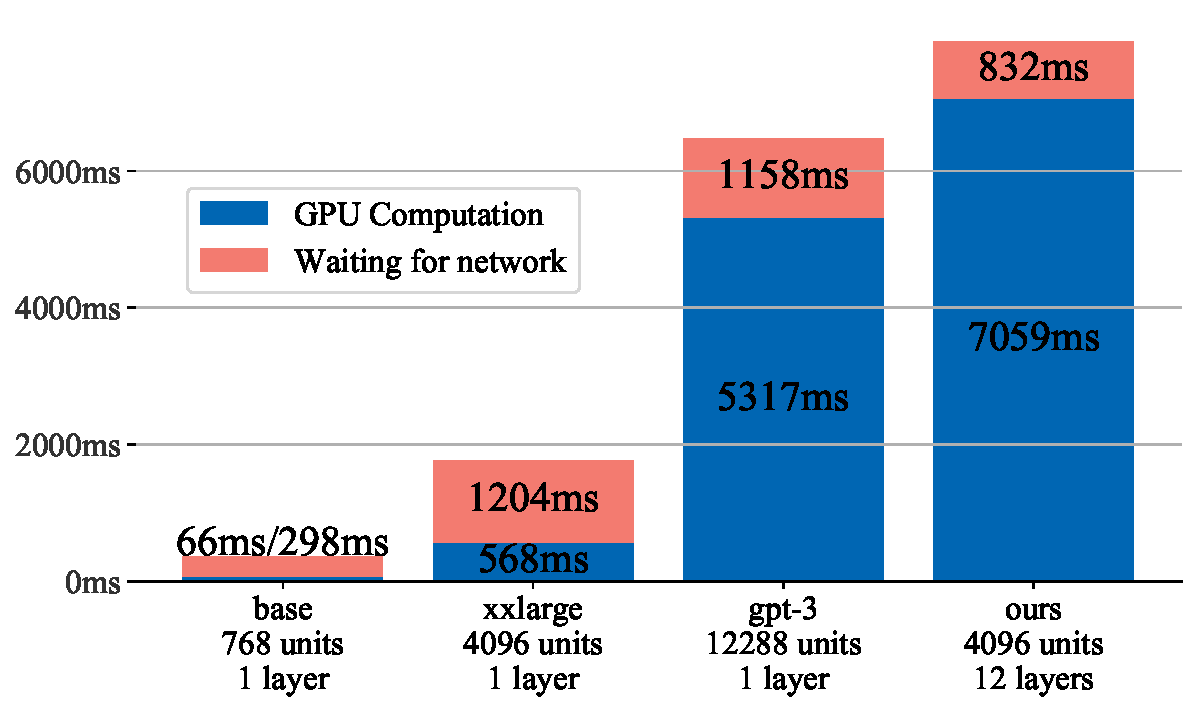
\includegraphics[width=1\linewidth]{resources/perf_absolute.pdf}
    \vspace{-12pt}
    \captionof{figure}{Pipeline computation and idle time per batch at 500 Mb/s bandwidth.}
    \label{fig:throughput_exps}
\end{figure}%
\begin{table}
    \centering
    \captionof{table}{Relative device utilization at 500 Mb/s bandwidth and varying network latency.}
    \label{tab:latency}
    \small
    \setlength{\tabcolsep}{8pt}
    \begin{tabular}[b]{@{}lcccc@{}}
    \toprule
    \multirow{2}{*}{\thead{Latency\\(RTT)}} & 
    \multicolumn{4}{c}{
    \thead{
    Relative GPU utilization\\ (100\% - idle time)
    }
    }
    
    \\
\cmidrule{2-5}                     & base & xxlarge & GPT-3 & Ours \\ \midrule
    None &   18.0\%     &  32.1\%         &  82.1\%  &  89.5\%      \\
    10ms &   11.8\%      &   28.9\%    &   79.3\%   &  87.2\%    \\
    50ms &    4.88\%      &   20.1\%    &   70.3\% &  79.5\%    \\
    100ms &    2.78\%      &    14.9\%    &  60.2\%     &   71.5\% \\
    200ms &   1.53\%     &  10.1\%    &  48.5\%   &     59.2\%    \\
    \bottomrule
    \end{tabular}
    \vspace{-6pt}
\end{table}

As depicted in Figure~\ref{fig:squarecube} (right) and Figure~\ref{fig:throughput_exps}, larger models achieve better GPU utilization rate in the same network conditions, since their communication load grows slower than computation. More importantly, even at 500 Mb/s, the resulting GPU idle time can be pushed into the 10--20\% range, either naturally for GPT-3-sized models or through activation compression for smaller models. In addition, large models maintain most of their training efficiency at the 100ms latency~(Table~\ref{tab:latency}), which is roughly equivalent to training on different continents~\citep{verizon_latency}.

\vspace{-4pt}
\subsection{Detailed Performance Comparison}\label{appendix:training_throughput}

Here we investigate how SWARM parallelism compares to existing systems for training large models: \textbf{GPipe}~\citep{huang2019gpipe} and \textbf{ZeRO-Offload}~\citep{zerooffload}.
The purpose of this section is to compare the training throughput in ``ideal'' conditions (with homogeneous reliable devices and balanced layers), as deviating from these conditions makes it \textit{infeasible} to train with baseline systems.
Still, even in such conditions the performance of different systems can vary across model architectures, and hence we want to identify the cases in which using SWARM is preferable to other approaches.
We benchmark individual SWARM components in preemptible setups in Section~\ref{sect:experiments_adaptive} and Appendix~\ref{appendix:scaling}.

We evaluate training performance for sequences of 4 Transformer layers of identical size distributed over 16 workers. Similarly to Section~\ref{sect:experiments_square_cube}, we use three layer configurations: ``xxlarge''~($d_{model} {=} 4096$, $d_{\text{FFN}} {=} 16384$, 32 heads), ``GPT-3''~($d_{model} {=} 12288$, $d_{\text{FFN}} {=} 49152$, 96 heads), and ``Ours''~($d_{model} {=} 4096$, $d_{\text{FFN}} {=} 16384$, 32 heads, 16 shared layers per block, last stage holds only the vocabulary projection layer). The microbatch size is 4 for ``xxlarge'' and 1 for ``GPT-3'' and ``Ours'', and the sequence length is 512.

To provide a more detailed view of the training performance, we measure two separate performance statistics: the training throughput and the All-Reduce time. 
The training throughput measures the rate at which the system can process training sequences, i.e., run forward and backward passes. 
More specifically, we measure the time required to process 6250 sequences of 512 tokens, which corresponds to the largest batch size used in~\citet{gpt3}.
In turn, the All-Reduce time is the time each system spends to aggregate accumulated gradients across devices. 
Intuitively, training with small batch sizes is more sensitive to the All-Reduce time (since the algorithm needs to run All-Reduce more frequently) and vice versa.


\textbf{Hardware setup:} Each worker uses a V100-PCIe GPU with 16 CPU threads (E5 v5-2660v4) and 128 GB RAM. The only exception is for ZeRO-Offload with ``GPT-3'' layers, where we had to double the RAM size because the system required 190 gigabytes at peak. Similarly to Section~\ref{sect:experiments_square_cube}, each worker can communicate at a 500 Mb/s bandwidth for both upload and download for a total of 1 Gb/s.
In terms of network latency, we consider two setups: with \textbf{no latency}, where workers communicate normally within the same rack, and with \textbf{latency}, where we introduce additional $100\pm50$ms latency directly in the kernel\footnote{More specifically, \texttt{tc qdisc add dev <...> root netem delay 100ms 50ms}}.

\textbf{GPipe configuration:} We use a popular PyTorch-based implementation of GPipe\footnote{The source code is available at \url{https://github.com/kakaobrain/torchgpipe}}. The model is partitioned into 4 stages repeated over 4 model-parallel groups. To fit into the GPU memory for the ``GPT-3'' configuration, we offload the optimizer into RAM using ZeRO-Offload. Before averaging, we use PyTorch's built-in All-Reduce to aggregate gradients.
We evaluate both the standard GPipe schedule and the 1F1B schedule~\citep{pipedream}.

\textbf{ZeRO-Offload configuration:} Each worker runs the entire model individually, then exchanges gradients with peers. For ``xxlarge'', we use the official implementation from~\cite{zerooffload}. However, for ``GPT-3'', we found that optimizer offloading still does not allow us to fit 4 layers into the GPU. For this reason, we also offload the model parameters using the \texttt{offload\_param} option.

\begin{table}
\centering
\small
\setlength{\tabcolsep}{4pt}
\captionof{table}{Training performance for different model sizes.}
\label{tab:throughput_gpt}
\begin{tabular}[b]{lcccc}
\toprule
\multirow{2}[2]{*}{System} &
  \multicolumn{2}{c}{Throughput, min/batch} &
  \multicolumn{2}{c}{All-Reduce time, min} \\ \cmidrule(lr){2-3}\cmidrule(lr){4-5} 
                 & No latency & Latency & No latency & Latency \\
 \midrule \multicolumn{5}{c}{``GPT-3'' (4 layers) }\\
 \midrule
SWARM            &  168.3 &\textbf{186.7}  &  7.4 & \textbf{7.6}   \\
GPipe            &  164.5 & 218.4 &  \multirow{2}{*}{\textbf{6.7}}    & \multirow{2}{*}{7.8}   \\
1F1B & \textbf{163.3} & 216.1 & & \\
Offload          &  272.7 & 272.7          &  25.5 & 27.3 \\
\midrule \multicolumn{5}{c}{``xxlarge'' (4 layers) }\\
\midrule
SWARM            &  44.2 & 48.2                  &  0.8  & \textbf{0.9}   \\
GPipe            &  40.1 & 108.8                  &  \multirow{2}{*}{\textbf{0.7}}  & \multirow{2}{*}{1.1}   \\
1F1B & 40.8 & 105.5 & & \\
Offload          &  \textbf{33.8} & \textbf{33.8}  &  2.8 & 4.2   \\
\midrule \multicolumn{5}{c}{Full ``Ours'' model (48 shared layers + embeddings) }\\
\midrule
SWARM            &  432.2 & 452.9                  &  0.8  &\bf 1.0   \\
GPipe            &  420.0 & 602.1                   &  \multirow{2}{*}{\bf 0.7}  & \multirow{2}{*}{1.1}   \\
1F1B             &  408.5 & 569.2 & & \\
Offload          &  \bf 372.0 &\bf 372.0  &  3.2 & 4.8   \\
\bottomrule
\end{tabular}
\vspace{-8pt}
\end{table}%

\begin{figure}[b]
\vspace{-16pt}
\centering
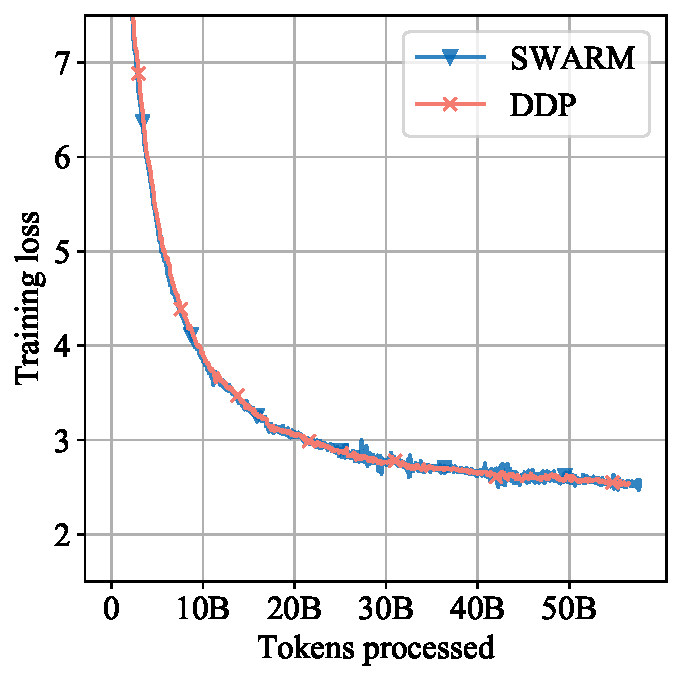
\includegraphics[ width=0.65\linewidth]{resources/learning_3stages.pdf}
\vspace{-6pt}
\captionof{figure}{Training convergence comparison.}
\label{fig:convergence}
\end{figure}

In turn, when training smaller models, ZeRO-Offload outperforms both SWARM and GPipe. This result aligns with our earlier observations in Figure~\ref{fig:squarecube}, where the same model spent most of the time waiting for the communication between pipeline stages.%

We also observe that ZeRO-Offload takes longer to aggregate gradients, likely because each peer must aggregate the entire model, whereas in SWARM and GPipe, peers aggregate a single pipeline stage. The variation between All-Reduce time in GPipe and SWARM is due to implementation differences. Overall, SWARM is competitive to HPC baselines even in an idealized homogeneous environment.

\subsection{Large-Scale Distributed Training}
\label{sect:experiments_large}

To verify the efficiency of SWARM parallelism in a practical scenario, we conduct a series of large-scale distributed experiments using preemptible (unreliable) cloud T4 and A100 GPUs over a public cloud network.

We train a Transformer language model with the architecture similar to prior work~\citep{gpt3,gptj,gptneo} and 1.01 billion parameters in total. Our model consists of 3 stages, each containing a single Transformer decoder block with $d_{model}=4096$ and 16 layers per pipeline stage. All workers within a stage serve the same group of layers, and all layers within each group use the same set of parameters, similarly to ALBERT~\citep{albert}. On top of this, the first stage also contains the embedding layer, and the last stage includes the language modeling head. Because of layer sharing, this model is equivalent to a 13B model from~\citet{gpt3} in terms of compute costs. 

We use 8-bit compression~\citep{adam8bit} for activations and gradients to reduce the communication intensity. Additional training setup details are covered in Appendix~\ref{appendix:detailed_large}.
SWARM nodes run rebalancing every $T=300$ seconds, and trainers measure peer performance using a moving average with $\alpha=0.1$. However, as we show in Section~\ref{sect:experiments_adaptive}, the throughput of SWARM is not very sensitive to the choice of these hyperparameters.



First, to verify that model parallelism with asynchronous updates does not have significant convergence issues, we train the model on the Pile~\citep{gao2020pile} dataset with 400 preemptible T4 instances, each hosting one accelerator. As a baseline, we use regular data-parallel training with offloading on 128 A100 GPUs.
We run both experiments for approximately 4 weeks and compare the learning curves.




Figure~\ref{fig:convergence} shows the results of this experiment: it can be seen that the training dynamics of two approaches are indeed similar, which demonstrates the viability of SWARM parallelism for heterogeneous and poorly-connected devices.

In the next experiment, we aim to measure the pipeline throughput in different hardware conditions and to compare it with an estimate of best-case pipeline performance.
We consider several setups: first, we use the same 400 preemptible T4 nodes; in another setup, we use 7 instances with 8 A100 GPU each; finally, we combine these fleets to create a heterogeneous setup. We examine the performance of the pipeline both with weight sharing and with standard, more common, Transformer blocks.

\begin{table}
\centering
\captionof{table}{Pipeline throughput, layer sharing.}
\label{tab:throughput}
\small
\begin{tabular}{@{}lcccc@{}}
\toprule
\multirow{2}{*}{\begin{tabular}[c]{@{}l@{}}Hardware\\ setup\end{tabular}} &
  \multicolumn{2}{c}{\begin{tabular}[c]{@{}c@{}}Throughput,\\ samples/s\end{tabular}} &
  \multicolumn{2}{c}{\begin{tabular}[c]{@{}c@{}}Optimal\\ bandwidth, Mb/s\end{tabular}} \\ \cmidrule(lr){2-3}\cmidrule(lr){4-5} 
                 & Actual & Best-case & Upload & Download \\ \midrule
T4           &  17.6      &   19.2        &   317.8     &     397.9     \\
A100          & 16.9       &   25.5        &   436.1     &     545.1     \\
T4 \& A100 &   27.3     &       ---    &   ---     &      ---    \\ \bottomrule
\end{tabular}
\end{table}
\begin{table}
\centering
\captionof{table}{Pipeline throughput, default Transformer.}
\label{tab:throughput_standard}
\small
\begin{tabular}{@{}lcc@{}}
\toprule
\multirow{2}{*}{\begin{tabular}[c]{@{}l@{}}Hardware\\ setup\end{tabular}} &
  \multicolumn{2}{c}{\begin{tabular}[c]{@{}c@{}}Throughput,\\ samples/s\end{tabular}} \\ \cmidrule(lr){2-3}
                 & Actual & Best-case \\ \midrule
T4           &  8.8      &   19.3        \\
A100          & 8.0       &   25.1        \\
T4 \& A100 &   13.4     &       ---    \\ \bottomrule
\end{tabular}
\end{table}






We measure the number of randomly generated samples processed by the pipeline both in our infrastructure and the ideal case that ignores all network-related operations (i.e., has infinite bandwidth and zero latency). The ideal case is emulated by executing a single pipeline stage 3 times locally on a single server and multiplying the single-node estimates by the number of nodes.

As demonstrated in the left two columns of Table~\ref{tab:throughput} and Table~\ref{tab:throughput_standard}, asynchronous training of compute-intensive models with 8-bit compressed activations regardless of the architecture specifics allows us to achieve high performance without a dedicated networking solution. Furthermore, the load balancing algorithm of SWARM allows us to dynamically and efficiently utilize different hardware without being bottlenecked by slower devices. 


Next, we use the same load testing scenario to estimate the bandwidth required to fully utilize each device type in the above infrastructure. For this, we measure the average incoming and outgoing bandwidth on the nodes that serve the intermediate stage of the pipeline. We summarize our findings in the right two columns of Table~\ref{tab:throughput}: it turns out that with layer sharing and 8-bit compression, medium-performance GPUs (such as T4) can be saturated even with moderate network speeds. Based on our main experiment, the optimal total bandwidth is roughly 100Mb/s higher than the values reported in Table 3 due to gradient averaging, loading state from peers, maintaining the DHT and streaming the training data.
Although training over the Internet with more efficient hardware might indeed underutilize the accelerator, this issue can be offset by advanced compression strategies such as compression-aware architectures or layer sharing, as shown in Table~\ref{tab:throughput}.

\begin{figure}[t]
    \centering
    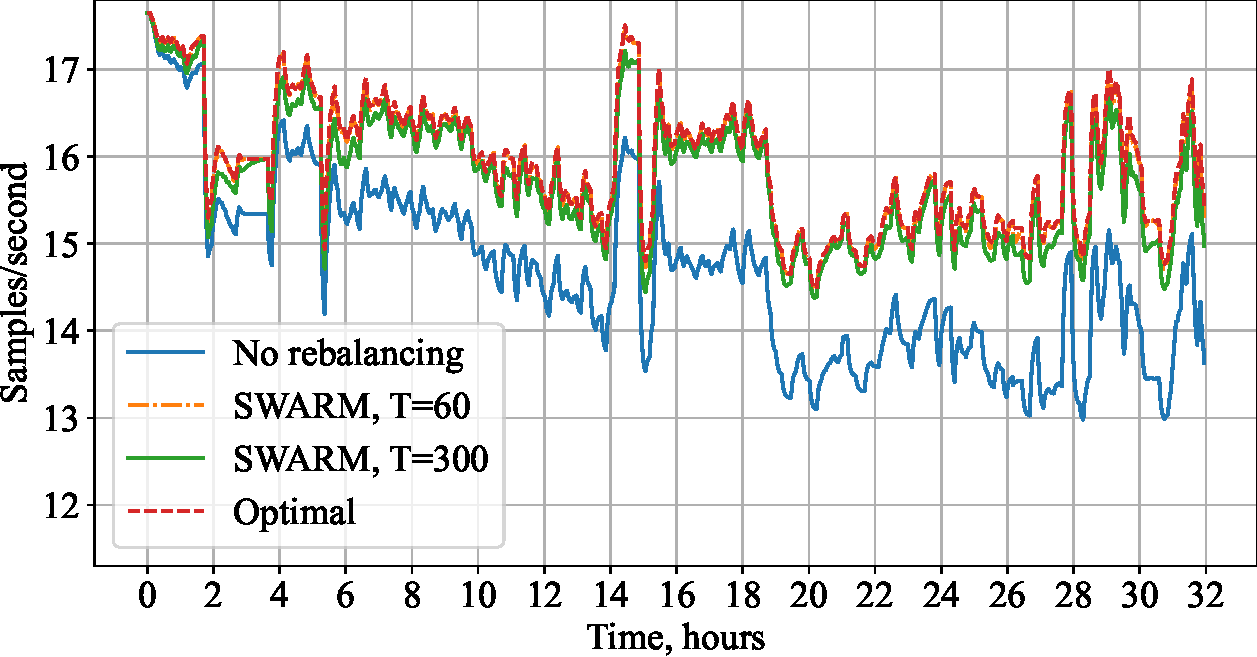
\includegraphics[width=\linewidth]{resources/rebalancing_activity.pdf}
    \captionof{figure}{Throughput of rebalancing methods over time.}
    \label{fig:rebalancing}
\end{figure}

\subsection{Adaptive Rebalancing Evaluation}


\begin{figure*}[h!]
\begin{subfigure}{0.5\textwidth}
    \centering
    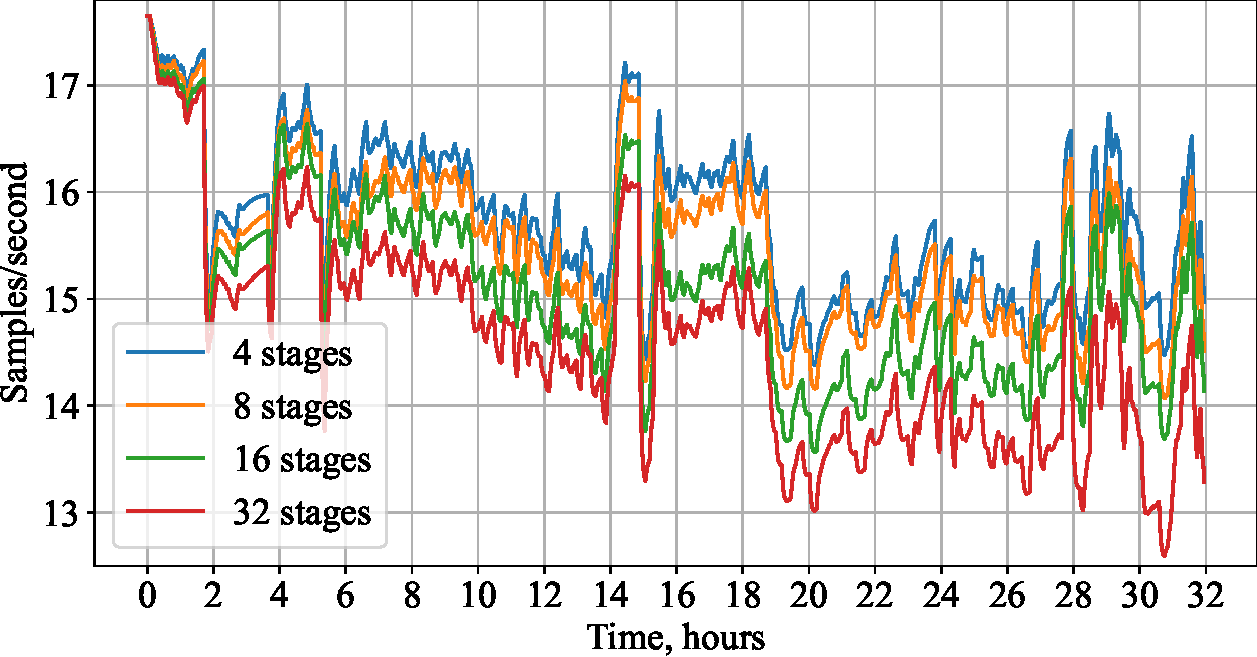
\includegraphics[width=0.97\linewidth]{resources/rebalancing_stages.pdf}
    \caption{Adaptive rebalancing of SWARM parallelism.}
    \label{fig:rebalancing_stages}
\end{subfigure}%
\begin{subfigure}{0.5\textwidth}
    \centering
    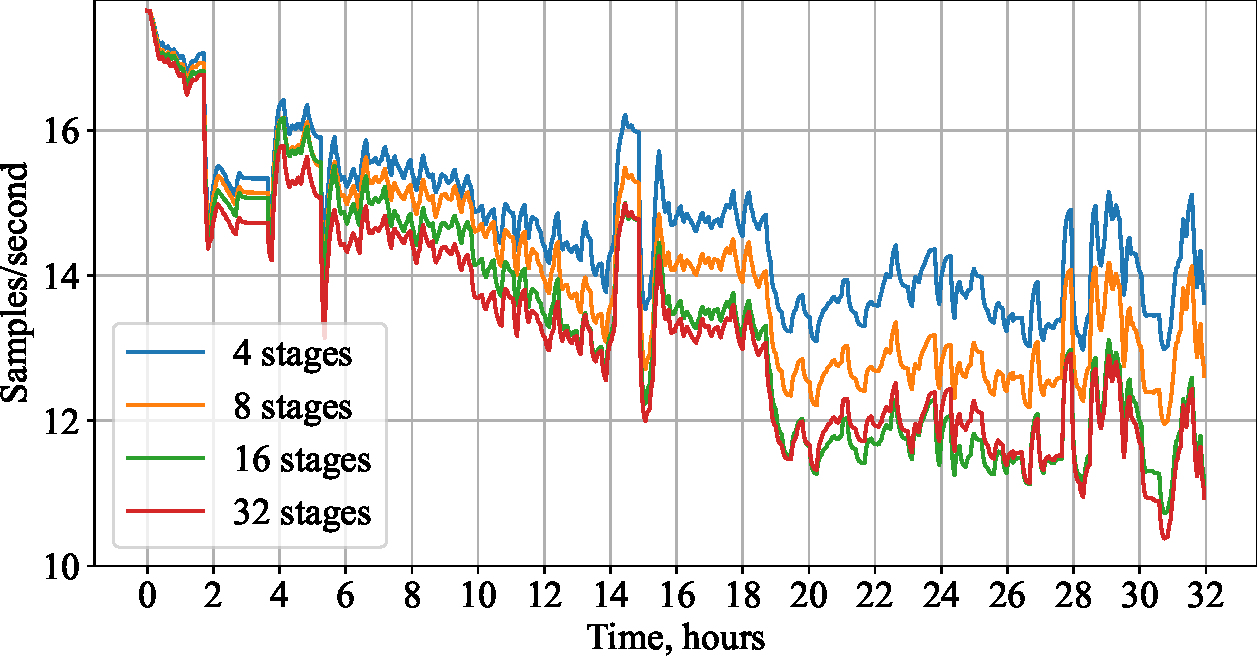
\includegraphics[width=0.97\linewidth]{resources/rebalancing_stages_baseline.pdf}
    \caption{No rebalancing.}
    \label{fig:rebalancing_stages_baseline}
\end{subfigure}
\caption{Scaling of pipeline-parallel strategies with respect to the number of stages.}
\label{fig:rebalancing_stages_all}
\end{figure*}

\label{sect:experiments_adaptive}
In this experiment, we evaluate the efficiency of adaptive peer rebalancing between stages proposed in Section~\ref{sect:method_swarm}. 
We use statistics of the number of active T4 nodes from the 32-hour segment of the experiment described in Section~\ref{sect:experiments_large}. 
We use this data to simulate training dynamics by viewing it as sequence of events, each consisting of a timestamp and a change in the number of peers (which can be positive or negative). 
When a worker is removed from the pipeline, we randomly choose the stage it was removed from: that is, removing $N$ peers corresponds to $N$ samples from the uniform distribution over four pipeline stages. 
We run 10 simulations with different random seeds and average the resulting trajectories.
We compare our strategy with two different values of $T$ to the baseline that has no rebalancing.

The results of this evaluation are available in \autoref{fig:rebalancing}; for reference, we also provide the performance of a theoretically optimal rebalancing strategy that maintains the highest possible throughput at every moment. It can be seen that even with the rebalancing period $T=300$, our approach significantly improves the overall throughput of the pipeline. When the number of peers is relatively stable, the rebalanced pipeline also approaches the optimal one in terms of throughput, which shows the efficiency of rebalancing even when moving only one node at a time.

In addition, we observed that for some brief periods, the performance of the unbalanced pipeline exceeded the throughput of the balanced one due to random choice of disconnecting peers (dropping more from the ``overrepresented'' stages affects the imbalanced pipeline less). However, this held true only for $\approx 4.5\%$ of the experiment and was quickly mitigated by adaptive rebalancing.

As expected, decreasing $T$ from 300 to 60 seconds improves both the overall throughput and the speed of convergence to optimal pipeline performance. However, the effect is not as drastic compared to the increase in DHT data transfer volume. This is also demonstrated by \autoref{tab:rebalancing_speedup}, which shows the relative throughput of the three configurations compared to the optimal one. Furthermore, the table displays that while initially there is little difference between rebalancing choices, it becomes more pronounced later on as the imbalanced version ``drifts further'' from the optimal state.

\begin{table}[b]
\centering
\captionof{table}{Relative throughput comparison of pipeline rebalancing methods.}
\small
\label{tab:rebalancing_speedup}
\begin{tabular}[b]{@{}lccc@{}}
\toprule
\multirow{2}[2]{*}{\thead{Rebalancing}} & \multicolumn{3}{c}{\% of optimal} \\ \cmidrule(l){2-4} 
                        & Overall   & First 1 hour   & Last 1 hour  \\ \midrule
None                & 82.7      & 99.0       & 45.4     \\
$T=300$    & 95.8      & 99.4       & 88.9     \\
$T=60$     & 97.6      & 99.8       & 91.7     \\ \bottomrule
\end{tabular}
\end{table}

Finally, we analyze the scaling properties of rebalancing with respect to the number of stages. To do this, we conduct experiments in the same setup as above ($T=300$) while changing the number of pipeline stages from 4 to $\{4,\ 8,\ 16,\ 32\}$. To ensure the consistency of throughput across all experiments, we increase the starting number of peers accordingly while keeping the preemption rate constant. As a baseline, we also evaluate the throughput of the pipeline that has no rebalancing.

Figure~\ref{fig:rebalancing_stages_all} shows the outcome of this experiment. As displayed in the plots, both strategies drop in performance with the increase in the stage count: while all stages should drop in performance equally in expectation, in practice, the variances are too large while the number of peers is relatively too small for the asymptotic properties to take place. This effect results in more outliers (large drops in the number of peers) in the preemption distribution for more stages. Still, rebalancing allows to partially mitigate the issue: while we observe a more consistent downward trend for the baseline strategy, the rebalanced pipeline regains its performance over time and achieves a higher overall throughput.


\section{Conclusion}
In this work, we advance the method of {machine unlearning} through a novel viewpoint: model sparsification, achieved by weight pruning. We show in both theory and practice that model sparsity plays a foundational and crucial role in closing the gap between exact unlearning and existing approximate unlearning methods. Inspired by that, we propose two new unlearning paradigms,  `prune first, then unlearn' and `sparsity-aware unlearn', which can significantly improve the efficacy of approximate unlearning. We demonstrate the effectiveness of our findings and proposals in extensive experiments across different unlearning setups. Our study also indicates the presence of \textit{model modularity} traits, such as weight sparsity, that could simplify the process of machine unlearning. This may open up exciting prospects for future research to investigate unlearning patterns within weight or architecture space.






%\begin{ack}
\label{acknowledge}
Use unnumbered first level headings for the acknowledgments. All acknowledgments
go at the end of the paper before the list of references. Moreover, you are required to declare
funding (financial activities supporting the submitted work) and competing interests (related financial activities outside the submitted work).
More information about this disclosure can be found at: \url{https://neurips.cc/Conferences/2024/PaperInformation/FundingDisclosure}.


Do {\bf not} include this section in the anonymized submission, only in the final paper. You can use the \texttt{ack} environment provided in the style file to automatically hide this section in the anonymized submission.
\end{ack}

%%%%%%%%%%%%%%%%%%%%%%%%%%%%%%%%%%%%%%%%%%%%%%%%%%%%%%%%%%%%
% Reference
\newpage
{
\small
\bibliographystyle{plainnat}
\bibliography{reference}
}
%%%%%%%%%%%%%%%%%%%%%%%%%%%%%%%%%%%%%%%%%%%%%%%%%%%%%%%%%%%%

% \input{texts/paper checklist}


% \setcounter{lemma}{0}
%     \renewcommand{\thelemma}{\Alph{section}\arabic{lemma}}
    
\begin{comment}
\end{comment}

{\colorred 
\section{Compatible Value Function}
\label{app:comp_v}

The original policy gradient with compatible value function is stated as follow. 
\begin{theorem}
[\cite{sutton1999policy}]
Let $Q_w$ be a state-action function with parameter $w$ and $\pi_\theta$ be a policy function with parameter $\theta$. 
If $Q_w$ satisfies $\mathbb{E}_{\pi} [(Q^\pi - Q_w) \nabla_w Q_w] = 0$ and 
$\nabla_w Q_w = \nabla_\theta \log \pi_\theta,$
then $$\nabla_\theta \mathcal{J} = \mathbb{E}_\pi [Q_w \nabla_\theta \log \pi_\theta].$$
\label{thm:pg_fa}
\end{theorem}
If we let $w = \theta$ in Theorem \ref{thm:pg_fa}, where $Q_w$ and $\pi_\theta$ share parameters, we have the following theorem. 
\begin{theorem}
Let $Q_\theta$ be a state-action function with parameter $\theta$ and $\pi_\theta$ be a policy function with parameter $\theta$. 
If $Q_\theta$ satisfies $\mathbb{E}_{\pi} [(Q^\pi - Q_\theta) \nabla_\theta Q_\theta] = 0$ and 
$\nabla_\theta Q_\theta = \nabla_\theta \log \pi_\theta,$
then $$\nabla_\theta \mathcal{J} = \mathbb{E}_\pi [Q_\theta \nabla_\theta \log \pi_\theta].$$
\label{thm:pg_fa2}
\end{theorem}
Define 
$$\chi \overset{def}{=} \mathbb{E}_\pi [\cos <\nabla_\theta Q_\theta, \nabla_\theta \log \pi_\theta>].$$
We show that $\chi = 1$ is the necessary condition for the compatible condition $\nabla_\theta Q_\theta = \nabla_\theta \log \pi_\theta$. 
\begin{theorem}
i) If $\nabla_\theta Q_\theta \propto \nabla_\theta \log \pi_\theta$ for all states, then $\chi = 1$.

ii) If $\chi = 1$, then $\nabla_\theta Q_\theta \propto \nabla_\theta \log \pi_\theta$ for all states. 
\label{thm:connect_cond}
\end{theorem}
By Theorem \ref{thm:connect_cond}, $\chi = 1$ is equivalent to $\nabla_\theta Q_\theta \propto \nabla_\theta \log \pi_\theta$, and $\nabla_\theta Q_\theta \propto \nabla_\theta \log \pi_\theta$ is the necessary condition for $\nabla_\theta Q_\theta = \nabla_\theta \log \pi_\theta$, hence $\chi = 1$ is the necessary condition for $\nabla_\theta Q_\theta = \nabla_\theta \log \pi_\theta$.
\begin{proof}
i) Since $\nabla_\theta Q_\theta \propto \nabla_\theta \log \pi_\theta$, we have $<\nabla_\theta Q_\theta, \nabla_\theta \log \pi_\theta> = 0$. 
By definition of $\chi$, we have 
$$\chi = \mathbb{E}_\pi [\cos <\nabla_\theta Q_\theta, \nabla_\theta \log \pi_\theta>] = \mathbb{E}_\pi [1] = 1.$$

ii) Since $\chi \leq 1$ and $\cos(x)$ is monotonic decreasing as $x$ goes from $0$ to $\pi$, the equality $\chi = 1$ only holds when all states satisfy $\cos <\nabla_\theta Q_\theta, \nabla_\theta \log \pi_\theta> = 0$, which means $\nabla_\theta Q_\theta \propto \nabla_\theta \log \pi_\theta$. 
\end{proof}
}

% $$
% \begin{aligned}
%     logp &= variable((3, 3, 4)) \\
%     q &= variable((3, 3, 4)) \\
%     alpha &= 0.3 \\
%     \pi &= softmax(alpha * logp + (1.0 - alpha) * q) \\
% \end{aligned}
% $$
\clearpage

\section{Gradients Between Policy Improvement and Policy Evaluation}
\label{app:mtv}

\begin{table}[hb!]
    \centering
    \scalebox{0.90}{
    \begin{math}
        \begin{array}{c|c|c|c}
    \toprule
     & \text{Function Approximation} & \text{Train Gradients} & \text{Cosine of Interested Angles} \\
    \midrule
    
    \text{PPO} & (V, logit) = (V_\theta, logit_\theta) & 0.5 \nabla L_V + \nabla \mathcal{J} & %\cos<\nabla L_V, \nabla \mathcal{J}> 
    \\ 
    & \pi = \text{softmax}(logit) & & \\
    
    \midrule
    
    \text{PPO ver.1} & (Q, logit) = (Q_\theta, logit_\theta), & 0.5 \nabla L_V + \nabla \mathcal{J} & \cos<\nabla L_Q, \nabla \mathcal{J}>%\cos<\nabla L_V, \nabla \mathcal{J}> 
    \\
    & \pi = \text{softmax}(logit) & & \cos<\nabla Q, \nabla \log \pi> \\
    & V = sg(\pi)\cdot Q & & %\cos<\nabla L_V, \nabla L_Q> 
    \\
    % & & &  \\
    
    \midrule
    
    \text{PPO ver.2} & (Q, logit) = (Q_\theta, logit_\theta), & 0.5 \nabla L_V + \nabla L_Q + \nabla \mathcal{J} & \cos<\nabla L_Q, \nabla \mathcal{J}> %\cos<\nabla L_V, \nabla \mathcal{J}> 
    \\
    & pi = \text{softmax}(logit) & & \cos<\nabla Q, \nabla \log \pi> \\
    & V = sg(\pi)\cdot Q & & %\cos<\nabla L_V, \nabla L_Q> 
    \\
    % & & &  \\
    
    \midrule
    
    \text{PPO+CASA} & (V, A) = (V_\theta, A_\theta), & 0.5 \nabla L_V + \nabla L_Q + \nabla \mathcal{J} & \cos<\nabla L_Q, \nabla \mathcal{J}> %\cos<\nabla L_V, \nabla \mathcal{J}> 
    \\
    & \pi = \text{softmax}(A/\tau), & & \cos<\nabla Q, \nabla \log \pi> \\
    & \Bar{A} = A - sg(\pi) \cdot A & & %\cos<\nabla L_V, \nabla L_Q> 
    \\
    & Q = \Bar{A} + sg(V) & &  \\
    
    \bottomrule 
    \end{array}
    \end{math}
    }
    
    \caption{PPO is the original PPO. PPO ver.1 and PPO ver.2 are adapted versions to calculate $\nabla L_Q$. PPO+CASA is applying CASA on PPO, which is described in Sec. \ref{sec:on_ppo_and_r2d2}.}
    \label{tab:ppo_mtv}
\end{table}

\begin{table}[ht!]
    \centering
    \scalebox{0.90}{
    \begin{math}
        \begin{array}{c|c|c|c}
    \toprule
     & \text{Function Approximation} & \text{Train Gradients} & \text{Cosine of Interested Angles} \\
    \midrule
    
    \text{R2D2} & (V, A) = (V_\theta, A_\theta) & \nabla L_Q & \cos<\nabla L_Q, \nabla \mathcal{J}>  %\cos<\nabla L_V, \nabla \mathcal{J}> 
    \\
    & Q = A + V & & \\
    & \pi = \text{softmax}(A / \tau) & & %\cos<\nabla L_V, \nabla L_Q> 
    \\
    % & & &  \\ % <\nabla Q, \nabla \log \pi>

    \midrule
    
    \text{R2D2 ver.1} & (V, A) = (V_\theta, A_\theta) & 0.5 \nabla L_V + \nabla L_Q & \cos<\nabla L_Q, \nabla \mathcal{J}>  % \cos<\nabla L_V, \nabla \mathcal{J}> 
    \\
    & Q = A + V & & % \cos<\nabla L_Q, \nabla \mathcal{J}> 
    \\
    & \pi = \text{softmax}(A / \tau) & & % \cos<\nabla L_V, \nabla L_Q> 
    \\
    % & & &  \\ % \cos<\nabla Q, \nabla \log \pi>

    \midrule
    
    \text{R2D2+CASA} & (V, A) = (V_\theta, A_\theta), & 0.5 \nabla L_V + \nabla L_Q + \nabla \mathcal{J} & \cos<\nabla L_Q, \nabla \mathcal{J}>  % \cos<\nabla L_V, \nabla \mathcal{J}> 
    \\
    & \pi = \text{softmax}(A/\tau),  & & %\cos<\nabla L_Q, \nabla \mathcal{J}> 
    \\
    & \Bar{A} = A - sg(\pi) \cdot A & & % \cos<\nabla L_V, \nabla L_Q> 
    \\
    & Q = \Bar{A} + sg(V) & &  \\ %\cos<\nabla Q, \nabla \log \pi>
    \bottomrule 
    \end{array}
    \end{math}
     }
    \caption{R2D2 is the original R2D2. R2D2 ver.1 is adapted version to include $\nabla L_V$ for training. R2D2+CASA is applying CASA on R2D2, which is described in Sec. \ref{sec:on_ppo_and_r2d2}.}
    \label{tab:r2d2_mtv}
\end{table}

To understand the behavior of 
{\colorred $$
    \beta \overset{def}{=} <\mathbb{E}_\pi[(Q^\pi-Q_\theta)\nabla_\theta Q_\theta],\, \mathbb{E}_\pi[(Q^\pi-V_\theta) \nabla_\theta \log \pi_\theta]>
$$
}
and 
{\colorred 
$$\chi \overset{def}{=} \mathbb{E}_\pi [\cos <\nabla_\theta Q_\theta, \nabla_\theta \log \pi_\theta>]$$
}
in reinforcement learning algorithms, we choose PPO as a representative for policy-based methods and R2D2 as a representative for value-based algorithms. 

Define $$L_V(\theta) = \mathbb{E}_\pi [ (V^{\pi} - V_\theta)^2 ],\  L_Q(\theta) = \mathbb{E}_\pi [ (Q^{\pi} - Q_\theta)^2 ],$$
and $$\nabla_\theta \mathcal{J}(\theta) = \mathbb{E}_\pi \left[ (Q^{\pi}  - V_\theta ) \nabla_\theta \log \pi \right].$$
We usually have above three kinds of loss functions in reinforcement learning, which aim to estimate the state values, state-action values and the policy. 
We do not talk about the estimations of $V^\pi$ and $Q^\pi$ as they are estimated as their usual way of PPO's and R2D2's. 
All hyperparameters are listed in Appendix \ref{app:hyperparameters}. 

{\colorred For brevity, we write 
$$\cos<\nabla Q, \nabla \log \pi> = \mathbb{E}_\pi [\cos <\nabla_\theta Q_\theta, \nabla_\theta \log \pi_\theta>],$$
and
$$
\begin{aligned}
    &\cos<\nabla L_Q, \nabla \mathcal{J}> = \cos<\mathbb{E}_\pi[(Q^\pi-Q_\theta)\nabla_\theta Q_\theta],\, \mathbb{E}_\pi[(Q^\pi-V_\theta) \nabla_\theta \log \pi_\theta]>, \\
    &\cos<\nabla L_V, \nabla \mathcal{J}> = \cos<\mathbb{E}_\pi[(V^\pi-V_\theta)\nabla_\theta V_\theta],\, \mathbb{E}_\pi[(Q^\pi-V_\theta) \nabla_\theta \log \pi_\theta]>, \\
    &\cos<\nabla L_V, \nabla L_Q> = \cos<\mathbb{E}_\pi[(V^\pi-V_\theta)\nabla_\theta V_\theta],\, \mathbb{E}_\pi[(Q^\pi-Q_\theta) \nabla_\theta Q_\theta]>. \\
\end{aligned}
$$}

The fact that PPO only has $\nabla_\theta L_V$ and $\nabla_\theta \mathcal{J}$ and R2D2 only has $\nabla_\theta L_Q$ is the main difficulty to track $\cos(\beta)$ and $\chi$. 
To solve the problem, we adjust PPO and R2D2 with different versions.

For PPO, we displace the estimation of $V_\theta$ by $sg(\pi)\cdot Q_\theta$, where $Q_\theta$ is estimated by function approximation and $V_\theta$ is estimated by taking the expectation of $Q_\theta$.
All versions of PPO are listed in Table \ref{tab:ppo_mtv}.

For R2D2, we point out that though we apply $\epsilon$-greedy to interact with environments, $\epsilon$ is only used for exploration and the final target policy of value-based methods is simply $\arg\max Q_\theta$. 
Because $\arg\max Q_\theta$ breaks the gradient, we use a surrogate policy to approximate the gradient of policy improvement. 
% \haosen{potential context, the necessity of measuring the policy gradient and ``entropy'' of the Q function is that R2D2's greedy policy changes rapidly, and the rapid change give R2D2 the implicit exploration ability. \citep{policychurn} }
Since R2D2 uses dueling structure and $\text{softmax}(A_\theta / \tau) = \text{softmax}(Q_\theta / \tau) \overset{\tau \rightarrow 0+}{\longrightarrow} \arg\max Q_\theta$, we use $\pi_{surrogate} = \text{softmax}(A_\theta / \tau)$ to calculate the policy gradient. 
We only use $\pi_{surrogate}$ on learner to calculate the gradient, where the policy that interacts with environments is still $\epsilon$-greedy. 
All versions of R2D2 are listed in Table \ref{tab:r2d2_mtv}.

% Results are shown in Figure \ref{fig:mtv_app}.


% \begin{figure}[hb!]
% % \centering
% 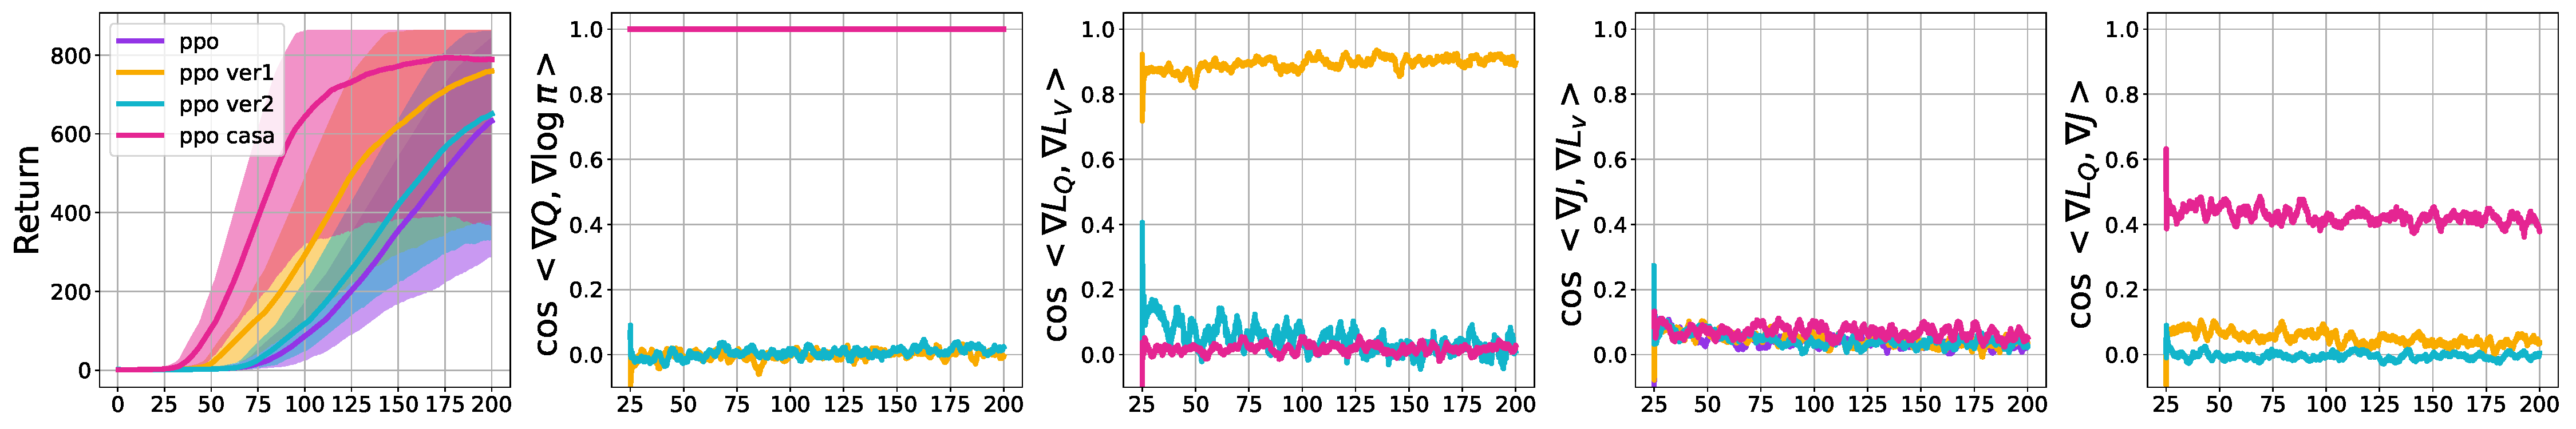
\includegraphics[width=\linewidth]{body/app_fig/app_ppo_Breakout.pdf}

% 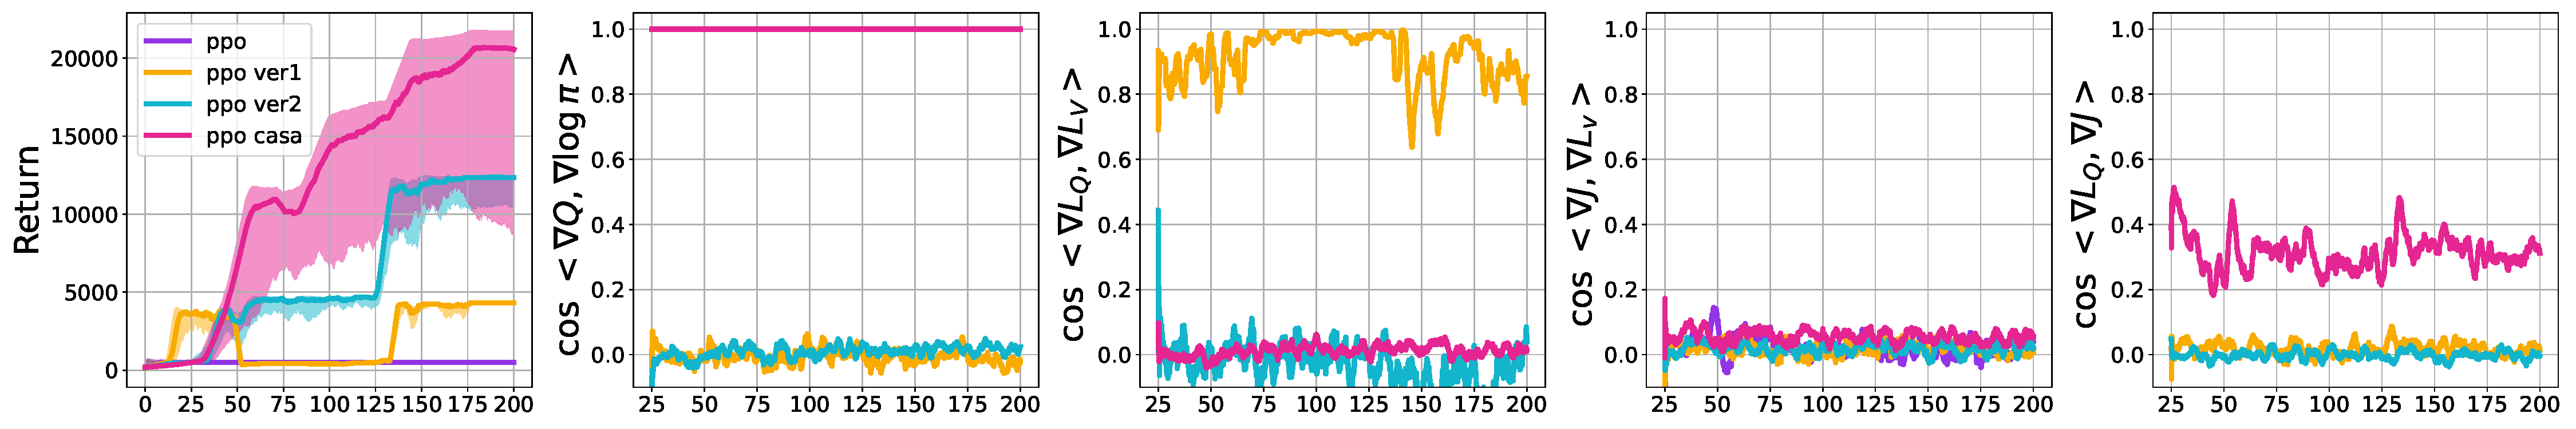
\includegraphics[width=\linewidth]{body/app_fig/app_ppo_Qbert.pdf}

% 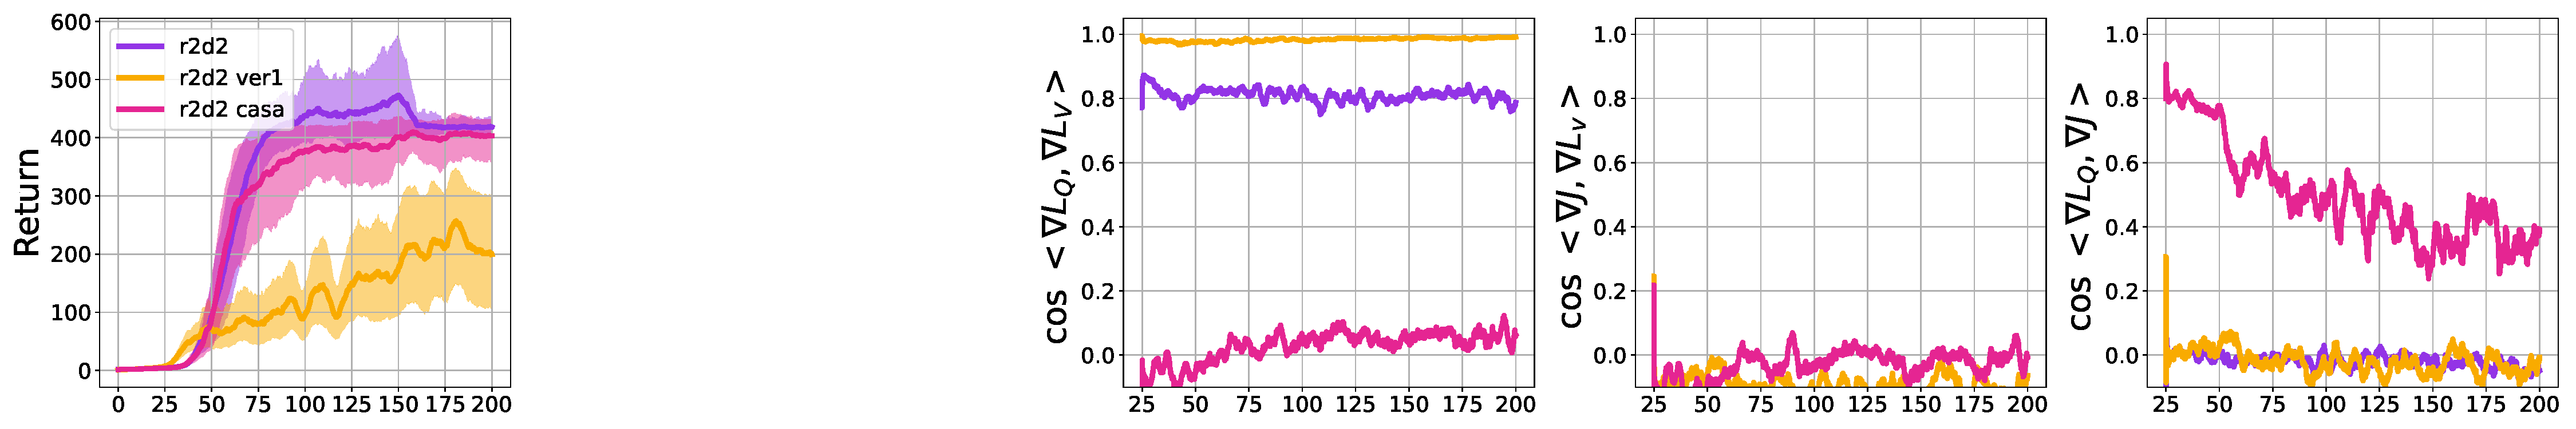
\includegraphics[width=\linewidth]{body/app_fig/app_r2d2_Breakout.pdf}


% 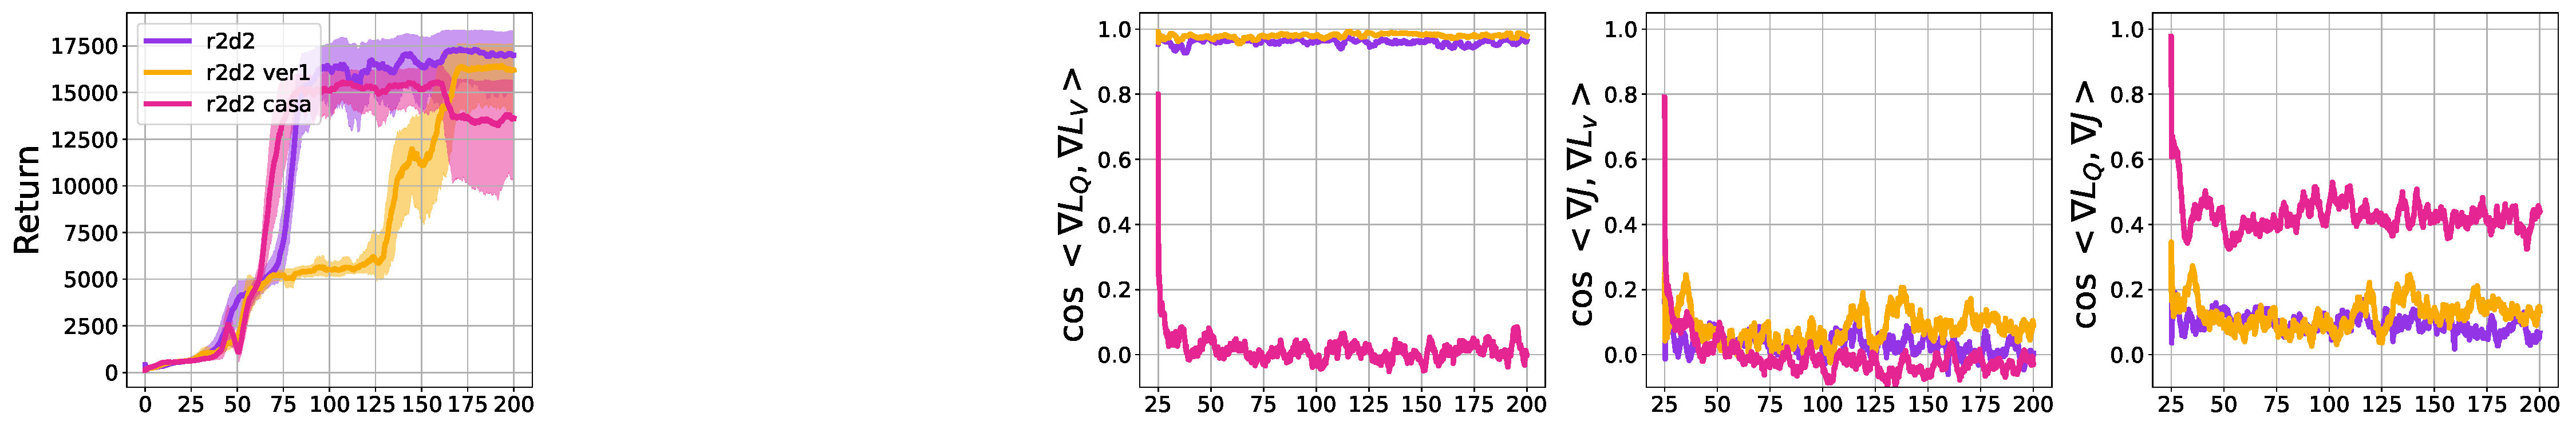
\includegraphics[width=\linewidth]{body/app_fig/app_r2d2_Qbert.pdf}
% \caption{Angles of Gradients and Returns of versions of PPO and R2D2 defined in Table \ref{tab:ppo_mtv} and Table \ref{tab:r2d2_mtv}.}
% \label{fig:mtv_app}
% \end{figure}

% \clearpage

% \changnan{casa summary deleted}
% \section{CASA summary}
% \begin{figure}[ht]
% \centering
% 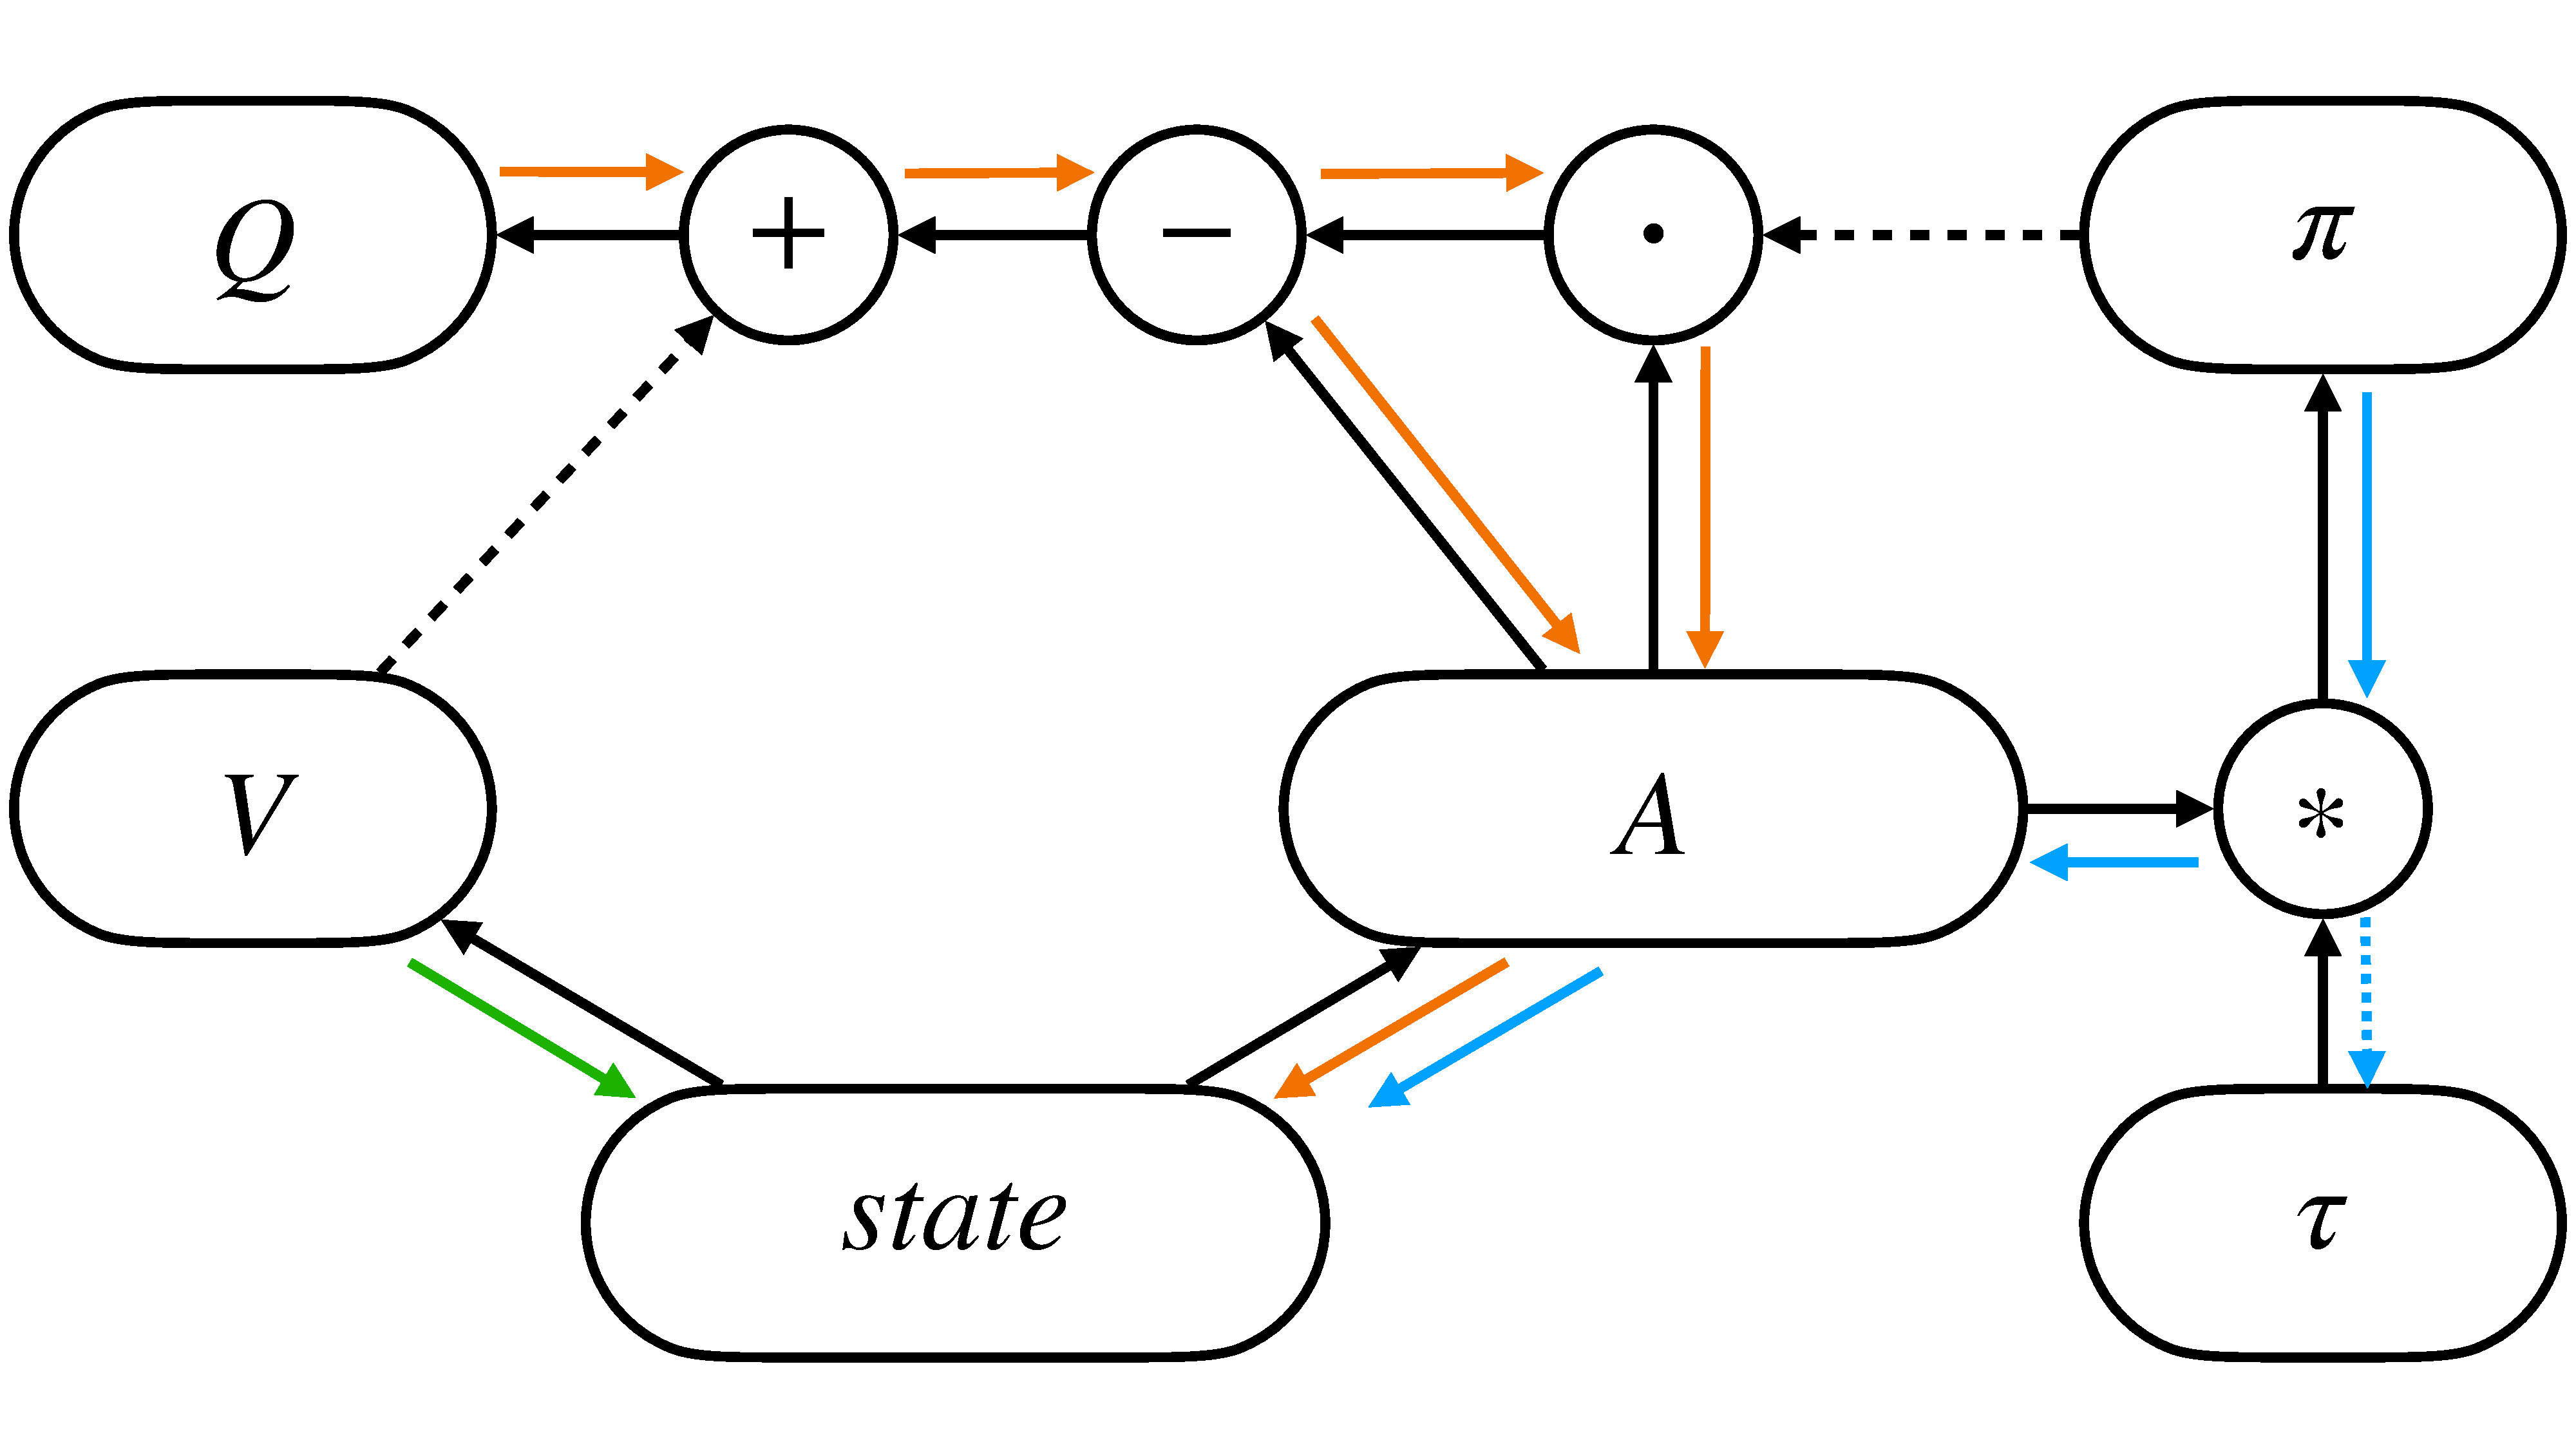
\includegraphics[width=0.4\textwidth,bb= 0 0 1800 1100]{body/figures/CASA.pdf}
% \caption{
% \textbf{Black} lines represent the forward process.
% \textbf{Dotted} black lines represent the \textit{stop gradient} operator in the forward process. 
% \textbf{Colorful} lines represent backpropagation from different loss functions. 
% Specifically, \textbf{blue} lines represent $\mathbb{E}_\pi [(Q^\pi-V)\nabla \log \pi]$, 
% \textbf{orange} lines represent $\mathbb{E}_\pi [(Q^\pi-Q)\nabla Q]$,
% and \textbf{green} lines represent $\mathbb{E}_\pi [(Q^\pi-V)\nabla V]$.}
% \label{fig:casa}
% \end{figure}
% \section{motivation experiments}

\clearpage

{\colorred \section{On Discussing Application of CASA on Continuous Action Space}
\label{app:cts_space}

As we can see CASA is only applied to discrete action space in the main context, we make a discussion on whether CASA is applicable on continuous action space. 
For brevity, we let $\tau=1$ and write \eqref{eq:casa} as:
\begin{equation}
\left\{
    \begin{aligned}
        &\pi = \text{softmax}(A), \\
        &\Bar{A} = A - \mathbb{E}_{\pi} [A], \\
        &Q = \Bar{A} + sg(V).
    \end{aligned}
\right. 
\end{equation}
The difficulty comes from estimating two quantities, one is $\text{softmax}(A)$, the other is $\mathbb{E}_{\pi} [A]$. 
This comes from the fact that discrete action space is countable so these two quantities are expressed in a closed-form, while continuous action space is uncountable so an accurate estimation of these two quantities is intractable. 
We can surely apply Monte Carlo methods to approximate, but a more elegant close-form expression may be preferred. 
Then this becomes another problem: \textit{how to estimate (state-action values / advantages / policy probabilities) of all actions in a continuous action space efficiently without loss of generality?}
This is another representational design problem, which is out of scope of this paper, so we don't touch much about it. 
But with the hope of inspiring a better solution to this problem, we provide one practical way of applying CASA on continuous action space based on kernel-based machine learning. 

Let $a_0, \dots, a_k$ to be basis actions in the action space. 
Let $A(s, a_0), \dots, A(s, a_k)$ to be advantage functions for tuples of states and basis actions. 
They can either share parameters or be isolated. 
Let $K(\cdot, \cdot)$ be a kernel function defined on the product of two action spaces. 
For any $a$ in the action space, we can estimate $A(s, a)$ by a decomposition such like $$A(s, a) = \frac{1}{Z_a} (K(a_0, a) A(s, a_0) + \dots + K(a_k, a) A(s, a_k)),$$ where $Z_a = \sum_{i=0}^k K(a_i, a)$ is a normalization constant. 

Since $K(\cdot, a)$ is a closed-form function of $a$, and $|\{A(s, a_0), \dots, A(s, a_k)\}|$ is finite, we can make a closed-form expression of both $\text{softmax}(A)$ and $\mathbb{E}_{\pi} [A]$. 
Then we can apply CASA directly on this expression, with one function estimates $V$ and the other function estimates advantages of all actions in a closed-form with only state as input.  
The policy is defined directly by $\text{softmax}$ of all advantages. 
In details, we define
\begin{equation}
\left\{
    \begin{aligned}
        &\pi(s, a) = \exp (A(s, a)) / \int_{a} \exp (A(s, a)) da, \\
        &\Bar{A}(s, a) = A(s, a) - \int_{a} sg(\pi(s, a)) A(s, a) da, \\
        &Q(s, a) = \Bar{A}(s, a) + sg(V(s)).
    \end{aligned}
\right. 
\end{equation}

Then it satisfies the consistency of CASA on continuous action space.
$$
\begin{aligned}
    \nabla \log \pi(s, a) &= \nabla A(s, a) - \frac{\nabla \int_{a} \exp (A(s, a)) da}{\int_{a} \exp (A(s, a)) da} \\
    &= \nabla A(s, a) - \frac{ \int_{a} \exp (A(s, a)) \nabla A(s, a) da}{\int_{a} \exp (A(s, a)) da} \\
    &= \nabla A(s, a) - \int_{a} \frac{  \exp (A(s, a)) }{\int_{a} \exp (A(s, a)) da} \nabla A(s, a) da \\
    &= \nabla A(s, a) - \int_{a} \pi(s, a) \nabla A(s, a) da \\
    &= \nabla \Bar{A}(s, a) = \nabla Q(s, a). 
\end{aligned}
$$
}

\section{DR-Trace}
\label{app:drtrace}

% One simple choice is to learn $V$ and $\pi$ by V-Trace \citep{impala} and to learn $Q$ by ReTrace \citep{retrace}. 
% \citep{impala} shows that $V^{\Tilde{\pi}}$ estimated by V-Trace converges to $V^*$ that corresponds to some $\Tilde{\pi}_{VTrace}$.
% Respectively, \citep{retrace} shows that $Q^{\Tilde{\pi}}$ estimated by ReTrace converges to $Q^*$ that corresponds to some $\Tilde{\pi}_{ReTrace}$.

As CASA estimates $(V, Q, \pi)$, we would ask
\textbf{i)} how to guarantee that $\Tilde{\pi}_{VTrace} = \Tilde{\pi}_{ReTrace}$, 
\textbf{ii)} how to exploit $(V, Q, \pi)$ to make a better estimation. 
Though we can apply V-Trace to estimate $V$ and ReTrace to estimate $Q$ with proper hyperparameters to guarantee $\Tilde{\pi}_{VTrace} = \Tilde{\pi}_{ReTrace}$, it's more reasonable to estimate $(V, Q)$ together. 
Inspired by Doubly Robust, which is shown to maximally reduce the variance, we introduce DR-Trace, which estimates $V$ by 
$$
\label{eq:dr-v}
    \begin{aligned}
        V_{DR}^{\Tilde{\pi}} (s_t) &\overset{def}{=} \mathbb{E}_{\mu} [ 
        V(s_t) + \sum_{k \geq 0} \gamma^k 
     c_{[t:t+k-1]} \rho_{t+k}  \delta^{DR}_{t+k} ],  
    \end{aligned}
$$
{\colorred where $\mu$ is the behavior policy}, $\delta^{DR}_t \overset{def}{=} r_t + \gamma V(s_{t+1}) - Q(s_t, a_t)$ is one-step Doubly Robust error, $\rho_t \overset{def}{=} \min\{\frac{\pi_t}{\mu_t}, \Bar{\rho} \}$ and $c_t \overset{def}{=} \min\{\frac{\pi_t}{\mu_t}, \Bar{c}\}$ are clipped per-step importance sampling, $c_{[t: t+k]} \overset{def}{=} \prod_{i=0}^{k} c_{t+i}$.

With one step Bellman equation, we estimate $Q$ by
$$
\label{eq:dr-q}
    \begin{aligned}
         Q_{DR}^{\Tilde{\pi}} (s_t, a_t) 
         &\overset{def}{=} \mathbb{E}_{s_{t+1}, r_t \sim p(\cdot, \cdot | s_t, a_t)} [  r_t + \gamma   V_{DR}^{\Tilde{\pi}} (s_{t+1}) ] 
        \\
        %  &=  \mathbb{E}_{\mu} [ r_t + \gamma V(s_{t + 1}) +
        % \gamma \sum_{k \geq 0} \gamma^k 
        % c_{[t+1:t+k]} \rho_{t+1+k}
        % \delta^{DR}_{t+1+k} V
        % ]
        % \\
        %  &= \mathbb{E}_{\mu}   [
        % Q(s_t, a_t) + \delta_t^{DR}V + \sum_{k \geq 1}  \gamma^k
        % c_{[t+1:t+k-1]} \rho_{t+k}
        % \delta^{DR}_{t+k} V
        % ],
        % \\
        &=  \mathbb{E}_{\mu}   [
        Q(s_t, a_t) + \sum_{k \geq 0}  \gamma^k
        c_{[t+1:t+k-1]} \Tilde{\rho}_{t, k}
        \delta^{DR}_{t+k}
        ], 
    \end{aligned}
$$
where $\Tilde{\rho}_{t, k} =  1_{\{k=0\}} + 1_{\{k > 0\}} \rho_{t+k}$.

% Compared to \eqref{eq:dr-v}, $c_{[t+1:t+k-1]} \Tilde{\rho}_{t, k}$ in \eqref{eq:dr-q} doesn't multiply importance sampling ratio of $a_t$, which meets the same intuition as \eqref{eq:vtrace} and \eqref{eq:retrace}.\\
\begin{theorem}
    Define $\Bar{A} = A - \mathbb{E}_\pi[A]$, $Q = \Bar{A} + sg(V)$,
    $$
    \begin{aligned}
    &\mathscr{T}(Q) \overset{def}{=} \mathbb{E}_{\mu}   [
        Q(s_t, a_t) + \sum_{k \geq 0}  \gamma^k
        c_{[t+1:t+k-1]} \Tilde{\rho}_{t, k}
        \delta^{DR}_{t+k}
        ], \\
    &\mathscr{S}(V) \overset{def}{=} \mathbb{E}_{\mu}   [
        V(s_t) + \sum_{k \geq 0}  \gamma^k
        c_{[t:t+k-1]} \rho_{t, k}
        \delta^{DR}_{t+k}
        ], \\
    &\mathscr{U}(Q, V) = (\mathscr{T}(Q) - \mathbb{E}_\pi[Q] + \mathscr{S}(V), \mathscr{S}(V)), \\
    &\mathscr{U}^{(n)}(Q, V) = \mathscr{U}(\mathscr{U}^{(n-1)}(Q, V)),
    \end{aligned}
    $$
    then $\mathscr{U}^{(n)}(Q, V) \rightarrow (Q^{\Tilde{\pi}}, V^{\Tilde{\pi}})$ that corresponds to 
    $$
        \Tilde{\pi}(a|s) = \frac
        {\min \left\{\Bar{\rho} \mu (a|s), \pi(a|s)\right\}}
        {\sum_{b \in \mathcal{A}}\min \left\{\Bar{\rho} \mu (b|s), \pi(b|s)\right\}}.
    $$ as $n \rightarrow +\infty$.
\label{thm:dr}
\end{theorem}
\begin{proof}
    See Appendix \ref{app:proof}, Theorem \ref{thm_app:dr}.
\end{proof}
Theorem \ref{thm:dr} shows that DR-Trace is a contraction mapping and $(V, Q)$ converges to $(V^{\Tilde{\pi}}, Q^{\Tilde{\pi}})$ that corresponds to 
$$
    \begin{aligned}
        \Tilde{\pi}(a|s) = \frac
        {\min \left\{\Bar{\rho} \mu (a|s), \pi(a|s)\right\}}
        {\sum_{b \in \mathcal{A}}\min \left\{\Bar{\rho} \mu (b|s), \pi(b|s)\right\}}.
    \end{aligned}
$$

% At training time, the policy evaluation is achieved by updating $\theta$ to minimize $l2$ losses
% $$
% \begin{aligned}
%     L_V(\theta) &= \mathbb{E}_\pi [ (V_\theta(s_t) -  V_{DR}^{\Tilde{\pi}} (s_t))^2 ], \\
%     L_Q(\theta) &= \mathbb{E}_\pi [ (Q_\theta(s_t, a_t) -  Q_{DR}^{\Tilde{\pi}} (s_t, a_t))^2 ],
% \end{aligned}
% $$ 
% which gives the ascent direction of $\theta$ by
% \begin{equation}
% \label{eq:grad_qv}
%     \begin{aligned}
%         \nabla_\theta L_V(\theta)
%         &= \mathbb{E}_\pi \left[ (V_{DR}^{\Tilde{\pi}} (s_t) - V_\theta(s_t) ) \nabla V_\theta(s_t) \right], \\
%         \nabla_\theta L_Q(\theta)
%         &= \mathbb{E}_\pi \left[ (Q_{DR}^{\Tilde{\pi}} (s_t, a_t) - Q_\theta(s_t, a_t)) \nabla Q_\theta(s_t, a_t) \right].
%     \end{aligned}
% \end{equation}
% And we make the policy improvement by policy gradient, which gives the ascent direction of $\theta$ by 
% \begin{equation}
% \label{eq:grad_pi}
% \begin{aligned}
%     \nabla_\theta \mathcal{J}(\tau, \theta) = \mathbb{E}_\mu \left[\tau \rho_t (Q_{DR}^{\Tilde{\pi}} (s_t, a_t) - V_\theta(s_t) ) \nabla_\theta \log \pi_t \right],
% \end{aligned}
% \end{equation}
% where $\mathcal{J} (\tau, \theta) = \tau \mathbb{E}_\pi [\sum \gamma^t r_t]$.
% It takes an additional $\tau$, which frees the scale of gradient from $\tau$.

% Finally, the gradient ascent direction of $\theta$ is given by
% \begin{equation}
%     \label{eq:grad_all}
%     \alpha_1 \nabla_\theta L_V + \alpha_2 \nabla_\theta L_Q + \alpha_3 \nabla_\theta \mathcal{J}.
% \end{equation}

% \textbf{Full algorithm is described in Appendix \ref{app:casa}.}
% Note that \eqref{eq:grad_all} doesn't need any entropy regularization. 
% We will discuss why this happens in section \ref{sec:equiv} and how CASA controls the exploration in section \ref{sec:ent_control}.


\begin{figure}[h]
    \centering
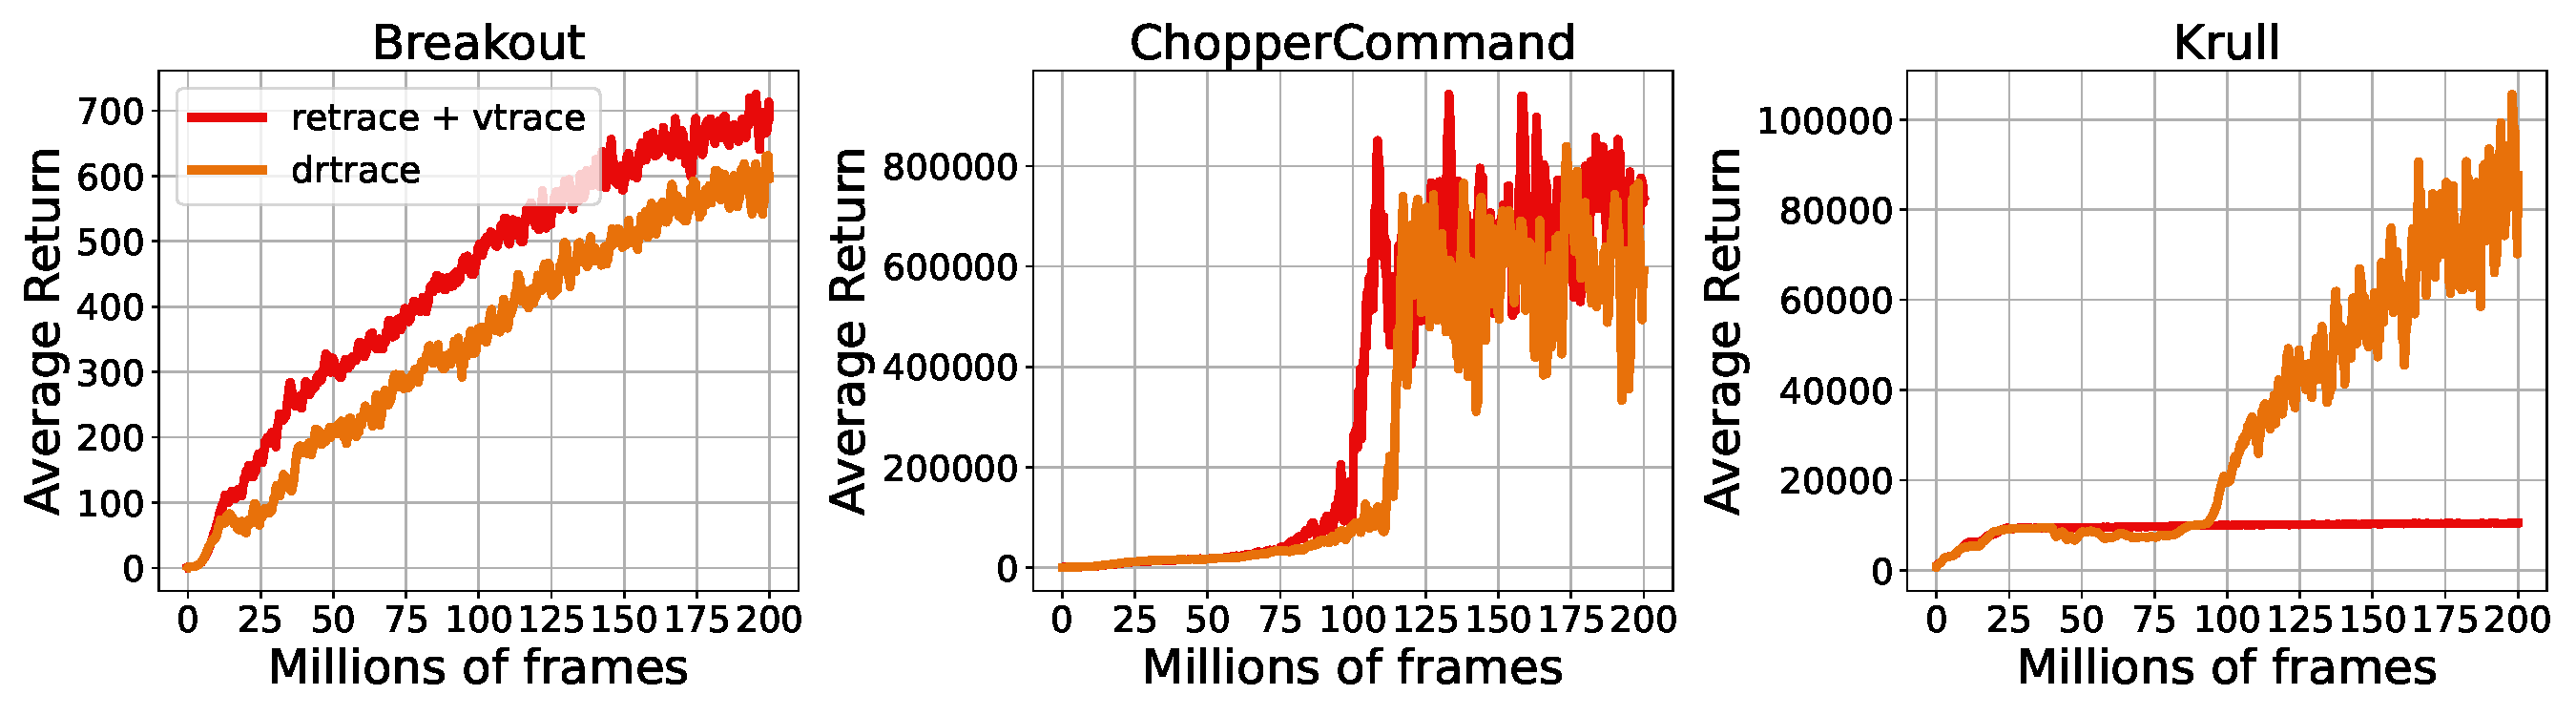
\includegraphics[width=\linewidth]{body/ablation/dr_ablation.pdf}
    \caption{Ablation study for w/wo DR-Trace on Breakout, ChopperCommand and Krull.}
    \label{fig:app_dr_trace}
\end{figure}

According to our proof, DR-Trace should work similar to V-Trace and ReTrace, as the convergence rate and the limitation are same. 
We compare DR-Trace with V-Trace+ReTrace in Figure \ref{fig:app_dr_trace}, where we replace estimation of state values by V-Trace and estimation of state-action values by ReTrace. 
We call V-Trace+ReTrace as No-DR-Trace for brevity. 
No-DR-Trace performs better on Breakout and ChopperCommand, but fails to make a breakthrough on Krull. 
Recalling the fact that Doubly Robust can maximally reduce the variance of Bellman error, No-DR-Trace is less stable but also potential to achieve a better performance. 
A conclusion cannot be made about No-DR-Trace, as this phenomenon means that No-DR-Trace is less stable than DR-Trace, but it also holds the potential to achieve a better performance.

% \clearpage


\section{Proofs}
\label{app:proof}

\theoremstyle{plain}
% \setcounter{Lemma}{0}
\newtheorem{Lemma_app}{Lemma}[section]
\newtheorem{Theorem_app}{Theorem}[section]
\theoremstyle{definition}
\newtheorem*{Remark_app}{Remark}
\theoremstyle{remark}

% \begin{Lemma_app}
% Let 
% $g \in \textbf{C}^{1}(\mathbb{R}^{n}): \mathbb{R}^{n} \to \mathbb{R}^{n}, \ f \in \textbf{C}^{1}(\mathbb{R}^{n+k}): \mathbb{R}^{n+k} \to \mathbb{R}^{n}.
% $\\
% If
% $
% \nabla_x g(x) = \nabla_x f(x, y)$, for $\forall x\in \mathbb{R}^{n}, y\in \mathbb{R}^k,
% $
% then $\exists$ $c \in \textbf{C}^{1}(\mathbb{R}^{k}): \mathbb{R}^{k} \to \mathbb{R}^{n}$, s.t. $f(x, y) = g(x) + c(y)$.
% \label{lemma_app:func_sep}
% \end{Lemma_app}
% \begin{proof}

% Let $\Tilde{f}(x, y) = f(x, y) - g(x)$.

% Since $\nabla_x g(x) = \nabla_x f(x, y)$, we have 
% $$
% \nabla_x \Tilde{f} = 0, \ for \ \forall x\in \mathbb{R}^{n}, y\in \mathbb{R}^k.
% $$

% So $\Tilde{f}$ is a constant function w.r.t $x$, which can be denoted as $c(y) = \Tilde{f}(x, y)$.

% Hence, $f(x, y) = g(x) + c(y)$.
% \end{proof}

\begin{Lemma_app}
(i) Define $\pi = softmax(A / \tau)$, then $\nabla \log \pi = (\textbf{1} - \pi) \frac{\nabla A}{\tau}$. 
(ii) Denote $sg$ to be stop gradient and define $\Bar{A} = A - \mathbb{E}_\pi [A]$, $Q = \Bar{A} + sg(V)$, then $\nabla Q = (\textbf{1} - \pi) \nabla A$.
\label{lemma_app:vannila_grad}
\end{Lemma_app}
\begin{proof}

As $Q = \Bar{A} + sg(V) = A - sg(\pi)\cdot A + sg(V)$, it's obvious that $\nabla Q = (\textbf{1} - \pi) \nabla A$.

For $\log \pi$, it's a standard derivative of cross entropy, so we have $\nabla \log \pi = (\textbf{1} - \pi) \nabla (A / \tau) = (\textbf{1} - \pi) \frac{\nabla A}{\tau}$.
\end{proof}

\begin{Lemma_app}
Define $\Bar{A}= A - \mathbb{E}_\pi[A]$, $Q = \Bar{A} + sg(V), \pi = softmax(A / \tau)$, then 
$$
\mathbb{E}_\pi \left[ (Q - V) \nabla \log \pi \right]
= - \tau \nabla \textbf{H}[\pi].
$$
\label{lemma_app:eqiv_pg_ent}
\end{Lemma_app}
\begin{proof}
Since 
$$
\pi = \exp(A / \tau) / Z,\ Z = \int_\mathcal{A} \exp(A / \tau),
$$
we have 
$$
A = \tau \log \pi + \tau \log Z.
$$
Based on the observation that $\mathbb{E}_\pi \left[ f(s) \nabla \log \pi (\cdot | s) \right] = 0$, 
we have 
$$\mathbb{E}_\pi \left[ \mathbb{E}_\pi[A] \cdot \nabla \log \pi \right] = 0,$$ 
$$\mathbb{E}_\pi \left[ \log Z \cdot \nabla \log \pi \right] = 0.$$

On the one hand,
$$
\begin{aligned}
    \mathbb{E}_\pi \left[ (Q - V) \nabla \log \pi \right]
    &= \mathbb{E}_\pi \left[ A \nabla \log \pi \right] 
    - \mathbb{E}_\pi \left[ \mathbb{E}_\pi[A] \cdot \nabla \log \pi \right] \\
    &= \tau \mathbb{E}_\pi \left[ \log \pi \nabla \log \pi \right]
    + \tau \mathbb{E}_\pi \left[ \log Z \cdot \nabla \log \pi \right] \\
    &= \tau \mathbb{E}_\pi \left[ \log \pi \nabla \log \pi \right].
\end{aligned}
$$

On the other hand, 
$$
\begin{aligned}
    \nabla \textbf{H} [\pi] 
    &= - \nabla \int_\mathcal{A} \pi_i \log \pi_i \\
    &= - \int_\mathcal{A}  \nabla \pi_i \cdot \log \pi_i - \int_\mathcal{A} \pi_i \nabla \log \pi_i  \\
    &= - \int_\mathcal{A}  \pi_i \nabla \log \pi_i \cdot \log \pi_i - \int_\mathcal{A}  \pi_i \frac{\nabla \pi_i}{\pi_i} \\
    &= - \mathbb{E}_\pi \left[ \log \pi \nabla \log \pi \right].
\end{aligned}
$$
Hence, $
\mathbb{E}_\pi \left[ (Q - V) \nabla \log \pi \right]
= - \tau \nabla \textbf{H}[\pi]
$.
\end{proof}

\begin{Theorem_app}
    Define $\Bar{A} = A - \mathbb{E}_\pi[A]$, $Q = \Bar{A} + sg(V)$.
    Define $$
    \begin{aligned}
    &\mathscr{T}(Q) \overset{def}{=} \mathbb{E}_{\mu}   [
        Q(s_t, a_t) + \sum_{k \geq 0}  \gamma^k
        c_{[t+1:t+k-1]} \Tilde{\rho}_{t, k}
        \delta^{DR}_{t+k}
        ], \\
    &\mathscr{S}(V) \overset{def}{=} \mathbb{E}_{\mu}   [
        V(s_t) + \sum_{k \geq 0}  \gamma^k
        c_{[t:t+k-1]} \rho_{t, k}
        \delta^{DR}_{t+k}
        ], \\
    &\mathscr{U}(Q, V) = (\mathscr{T}(Q) - \mathbb{E}_\pi[Q] + \mathscr{S}(V), \mathscr{S}(V)), \\
    &\mathscr{U}^{(n)}(Q, V) = \mathscr{U}(\mathscr{U}^{(n-1)}(Q, V)),
    \end{aligned}
    $$
    then $\mathscr{U}^{(n)}(Q, V) \rightarrow (Q^{\Tilde{\pi}}, V^{\Tilde{\pi}})$ that corresponds to 
    $$
        \Tilde{\pi}(a|s) = \frac
        {\min \left\{\Bar{\rho} \mu (a|s), \pi(a|s)\right\}}
        {\sum_{b \in \mathcal{A}}\min \left\{\Bar{\rho} \mu (b|s), \pi(b|s)\right\}}.
    $$ as $n \rightarrow +\infty$.
\label{thm_app:dr}
\end{Theorem_app}
\begin{Remark_app}
$\mathscr{T}(Q) - \mathbb{E}_\pi[Q] + \mathscr{S}(V)$ is \textbf{exactly} how $Q$ is updated at training time. 
Since $Q = \Bar{A} + sg(V)$, if we apply gradient ascent on $Q$ and $V$ in directions $\nabla L_Q(\theta)$ and $\nabla L_V(\theta)$ respectively, change of $Q$ comes from two aspects. One comes from $\nabla L_Q(\theta)$, which changes $A$, the other comes from $\nabla L_V(\theta)$, which changes $V$. Because the gradient of $V$ is stopped when estimating $Q$, the latter is captured by "minus old baseline, add new baseline", which is $- \mathbb{E}_\pi[Q] + \mathscr{S}(V)$ in Theorem \ref{thm_app:dr}.
\end{Remark_app}
\begin{proof}
 Define
 $$
 \begin{aligned}
        \widetilde{\mathscr{T}}(Q) &= - \mathbb{E}_\pi[Q] + \mathscr{T}(Q), \\
        \widetilde{\mathscr{U}}(Q, V) &= (\widetilde{\mathscr{T}}(Q), \mathscr{S}(V)), \\
        \widetilde{\mathscr{U}}^{(n)}(Q, V) &=   \widetilde{\mathscr{U}}(\widetilde{\mathscr{U}}^{(n-1)}(Q, V)).
 \end{aligned}
 $$
By Lemma \ref{lemma_app:dr_q}, $\widetilde{\mathscr{T}}^{(n)}(Q)$ converges to some $A^*$ as $n \rightarrow \infty$. This process will not influence the estimation of $V$ as the gradient of $V$ is stopped when estimating $Q$. According to the proof, $A^*$ does not depend on $V$. \\
By Lemma \ref{lemma_app:dr_v}, $\mathscr{S}^{(n)}(V)$ converges to some $V^*$ as $n \rightarrow \infty$. \\
Hence, we have
$$
\widetilde{\mathscr{U}}^{(n)}(Q, V) \rightarrow (A^*, V^*)\ \ as\ \ n \rightarrow +\infty. 
$$
By definition, 
$$
\mathscr{U}(Q, V) = (\widetilde{\mathscr{T}}(Q) + \mathscr{S}(V), \mathscr{S}(V)),
$$
we can regard $\widetilde{\mathscr{T}}(Q) + \mathscr{S}(V)$ as $Q$ and regard $\mathscr{S}(V)$ as $V$, then
$$
\begin{aligned}
    \mathscr{U}^{(2)}(Q, V) 
    &= \mathscr{U}(\widetilde{\mathscr{T}}(Q) + \mathscr{S}(V), \mathscr{S}(V)) \\
    &= (\mathscr{T}(\widetilde{\mathscr{T}}(Q) + \mathscr{S}(V)) -\mathscr{S}(V) + \mathscr{S}^{(2)}(V), \mathscr{S}^{(2)}(V)) \\
    &= (\widetilde{\mathscr{T}}^{(2)}(Q) + \mathscr{S}^{(2)}(V), \mathscr{S}^{(2)}(V)).
\end{aligned}
$$
By induction, 
$$
\begin{aligned}
    \mathscr{U}^{(n)}(Q, V) &= (\widetilde{\mathscr{T}}^{(n)}(Q) + \mathscr{S}^{(n)}(V), \mathscr{S}^{(n)}(V)) \\
    &\rightarrow (A^*+V^*, V^*)\ \ as\ \ n\rightarrow + \infty.
\end{aligned}
$$
Same as \citep{impala}, 
$$
    \Tilde{\pi}(a|s) = \frac
    {\min \left\{\Bar{\rho} \mu (a|s), \pi(a|s)\right\}}
    {\sum_{b \in \mathcal{A}}\min \left\{\Bar{\rho} \mu (b|s), \pi(b|s)\right\}}.
$$ 
is the policy s.t. the Bellman equation holds, which is 
$$\mathbb{E}_\mu[\rho_t (r_t + \gamma V_{t+1} - V_t) | \mathscr{F}_t] = 0,$$ and $\mathscr{U}(Q^{\Tilde{\pi}}, V^{\Tilde{\pi}}) = (Q^{\Tilde{\pi}}, V^{\Tilde{\pi}})$. \\
So we have
$(A^*+V^*, V^*) = (Q^{\Tilde{\pi}}, V^{\Tilde{\pi}}).$
\end{proof}

\begin{Lemma_app}
Define $\Bar{A}= A - \mathbb{E}_\pi[A]$, $Q = \Bar{A} + sg(V)$,
then operator 
$$
    \mathscr{T}(Q) \overset{def}{=} \mathbb{E}_{\mu}   [
        Q(s_t, a_t) + \sum_{k \geq 0}  \gamma^k
        c_{[t+1:t+k-1]} \Tilde{\rho}_{t, k}
        \delta^{DR}_{t+k}
        ]
$$
is a contraction mapping w.r.t. $Q$.
\label{lemma_app:dr_q}
\end{Lemma_app}
\begin{Remark_app}
Note that $\mathscr{T}(Q)$ is exactly \eqref{eq:dr-q}. 

Since $Q = A + sg(V)$, the gradient of $V$ is stopped when estimating $Q$, updating $Q$ will not change $V$, which is equivalent to updating $A$.
Without loss of generality, we assume $V$ is fixed as $V^*$ in the proof.
\end{Remark_app}
\begin{proof}

$\Bar{A} = A - \mathbb{E}_\pi[A]$ shows $\mathbb{E}_\pi[\Bar{A}] = 0$, which guarantees that no matter how we update $A$, we always have $\mathbb{E}_\pi[Q] = V^*$.

Based on above observations, define 
$$
    \widetilde{\mathscr{T}}(Q) \overset{def}{=} - \mathbb{E}_\pi [Q] + \mathscr{T}(Q).
$$

It's obvious that we only need to prove $\widetilde{\mathscr{T}}(Q)$ is a contraction mapping.

For brevity, we denote $$Q_t = Q(s_t, a_t), A_t = A(s_t, a_t), V^*_t = V^*(s_t).$$

Noticing that $\Tilde{\rho}_{t, 0} = 1$, let $\mathscr{F}$ represent filtration, we can rewrite $\widetilde{\mathscr{T}}$ as 
\begin{equation}
\label{eq:dr_a_2}
\begin{aligned}
    \widetilde{\mathscr{T}}(Q)
    &= \mathbb{E}_{\mu}   [
        A_t + \sum_{k \geq 0}  \gamma^k
        c_{[t+1:t+k-1]} \Tilde{\rho}_{t, k}
        \delta^{DR}_{t+k}
        ] \\
    &= \mathbb{E}_{\mu}   [
        -V^*_t + \sum_{k \geq 0}  \gamma^k
        c_{[t+1:t+k-1]} \Tilde{\rho}_{t, k}
        r_{t+k}
        + 
        \sum_{k \geq 0}  \gamma^{k+1}
        c_{[t+1:t+k-1]} \Delta_k ],
        \\
\end{aligned}
\end{equation}
where 
\begin{equation}
\label{eq:dr_delta}
    \Delta_k = \mathbb{E}_{\mu}\left[\Tilde{\rho}_{t, k} V^*_{t+k+1} - c_{t+k} \Tilde{\rho}_{t, k+1} Q_{t+k+1} | \mathscr{F}_{t+k}\right].
\end{equation}
By definition of $Q$,
$$
    \mathbb{E}_{\mu}[V_{t+k+1}^*|\mathscr{F}_{t+k}] 
    = \mathbb{E}_{\mu}[
    \mathbb{E}_\pi[Q_{t+k+1}|\mathscr{F}_{t+k+1}]
    |\mathscr{F}_{t+k}], \\
    % \geq&  \mathbb{E}_{\mu}[
    % \mathbb{E}_\mu[\Tilde{\rho}_{t, k+1} Q_{t+k+1}|\mathscr{F}_{t+k+1}]
    % |\mathscr{F}_{t+k}], 
$$
we can rewrite \eqref{eq:dr_delta} as
\begin{equation}
\label{eq:dr_q_delta}
\Delta_k = \mathbb{E}_{\mu}[
(
\Tilde{\rho}_{t, k} \frac{\pi_{t+k+1}}{\mu_{t+k+1}}- c_{t+k} \Tilde{\rho}_{t, k+1} 
) Q_{t+k+1} | \mathscr{F}_{t+k}
].
\end{equation}
For any $Q_1 = A_1 + sg(V^*)$, $Q_2 = A_2 + sg(V^*)$, since
$$
\mathbb{E}_{\mu}[
(
\Tilde{\rho}_{t, k} \frac{\pi_{t+k+1}}{\mu_{t+k+1}}- c_{t+k} \Tilde{\rho}_{t, k+1} 
) | \mathscr{F}_{t+k}
] \geq 0,
$$
by \eqref{eq:dr_a_2} \eqref{eq:dr_q_delta}, we have 
% $$
% || \Delta^1_k - \Delta_k^2 || \leq \mathbb{E}_{\mu}\left[
% \left(
% \Tilde{\rho}_{t, k} \frac{\pi_{t+k+1}}{\mu_{t+k+1}}- c_{t+k} \Tilde{\rho}_{t, k+1} 
% \right) | \mathscr{F}_{t+k}
% \right] ||A^1 - A_2||.
% $$
$$
        || \widetilde{\mathscr{T}}(Q_1) - \widetilde{\mathscr{T}}(Q_2) || 
        % \leq& \mathbb{E}_{\mu} \left[ \sum_{k \geq 0}  \gamma^{k+1} c_{[t+1:t+k-1]} || \Delta_k^1 - \Delta_k^2 || \right] \\
        \leq \mathcal{C} || Q_1 - Q_2 ||,
$$
where 
$$
    \begin{aligned}
        \mathcal{C} 
        &= \mathbb{E}_{\mu} [ \sum_{k \geq 0}  \gamma^{k+1} c_{[t+1:t+k-1]} 
        (
        \Tilde{\rho}_{t, k} \frac{\pi_{t+k+1}}{\mu_{t+k+1}}- c_{t+k} \Tilde{\rho}_{t, k+1} 
        ) ]
        \\
        &= \mathbb{E}_{\mu} [1 -1 + \sum_{k \geq 0}  \gamma^{k+1} c_{[t+1:t+k-1]} 
        \left(
        \Tilde{\rho}_{t, k} - c_{t+k} \Tilde{\rho}_{t, k+1} 
        \right) ] 
        \\
        &= 1 - (1 - \gamma)  \mathbb{E}_{\mu} [\sum_{k \geq 0} \gamma^{k}c_{[t+1:t+k-1]} \Tilde{\rho}_{t, k}  ] \\
        &\leq 1 - (1 - \gamma) < 1.
    \end{aligned}
$$
Hence, $\widetilde{\mathscr{T}}(Q)$ is a contraction mapping and converges to some fixed function, which we denote as $A^*$. So $\mathscr{T}(Q)$ is also a contraction mapping and converges to $A^*+V^*$.
\end{proof}

\begin{Lemma_app}
Define $Q = A + sg(V)$ with $\mathbb{E}_\pi [A] = 0$,
then operator 
$$
    \mathscr{S}(V) \overset{def}{=} \mathbb{E}_{\mu}  [
        V(s_t) + \sum_{k \geq 0}  \gamma^k
        c_{[t:t+k-1]} \rho_{t, k}
        \delta^{DR}_{t+k}
        ]
$$
is a contraction mapping w.r.t. $V$.
\label{lemma_app:dr_v}
\end{Lemma_app}
\begin{Remark_app}
Note that $\mathscr{S}(V)$ is exactly \eqref{eq:dr-v}. 
\end{Remark_app}
\begin{proof}

% Since $Q = A + sg(V)$, updating $V$ wouldn't influence $A$. WLOG, we assume $A$ is fixed as $A^*$ in Lemma \ref{lemma_app:dr_v}. \\
Same as Lemma \ref{lemma_app:dr_q}, we can get
$$
    \Delta_k = \mathbb{E}_{\mu}\left[
    \left( \rho_{t+k} - c_{t+k} \rho_{t+k+1}\right) V_{t+k+1} 
     -  c_{t+k} \rho_{t+k+1} A^*_{t+k+1} | \mathscr{F}_{t+k}\right],
$$
so we have 
$$
    \Delta^1_k - \Delta^2_k = \mathbb{E}_{\mu}\left[ 
    \left( \rho_{t+k} - c_{t+k} \rho_{t+k+1}\right) \cdot  
   (V^1_{t+k+1} -  V^2_{t+k+1})
     | \mathscr{F}_{t+k}\right].
$$
The remaining proof is identical to \citep{impala}'s.
\end{proof}

% \clearpage

% \begin{Lemma_app}
% Let $v \in \mathbb{R}^{|\mathcal{A}|}$ to be a vector. 
% Define 
% $
%     \pi (\tau) = \exp (v / \tau) / Z,\  Z = \int_\mathcal{A}  \exp(v / \tau).
% $
% Let $\Omega$ to be a probability measure supported on $[K, +\infty]$,
% then $f(\Omega) = \mathbb{E}_{\tau \sim \Omega} [\mathbb{E}_{\pi(\tau)} [v]]$ satisfies Lipschitz-1 condition with Wasserstein-1 metric.
% \label{lemma_app:lips}
% \end{Lemma_app}
% \begin{proof}
% Without loss of generality, we assume $v_1 \geq v_2 \geq ... \geq v_{|\mathcal{A}|}$.

% For any $\tau \in [0, +\infty)$, since
% $$
% \begin{aligned}
%     \pi (\tau) = \exp (v / \tau) / Z,\  Z = \int_\mathcal{A}  \exp(v / \tau),
% \end{aligned}
% $$
% we have
% $$
%     v = \tau \log \pi (\tau) + \tau \log Z.
% $$

% Denote $\Tilde{v}_j = v_j / \tau$. \\
% Since 
% $$
% \frac{\partial \log \pi_i}{\partial \Tilde{v}_j} = 1_{i=j} - \pi_j,
% $$
% we have
% $$
% \begin{aligned}
%     \frac{\partial \log \pi_i}{\partial \tau} 
%     &= \sum_j \frac{\partial \log \pi_i}{\partial \Tilde{v}_j} \cdot \frac{\partial \Tilde{v}_j}{\partial \tau} \\
%     &= - \sum_j (1_{i=j} - \pi_j) \frac{v_j}{\tau^2} \\
%     &= - \frac{1}{\tau^2} ( v_i - \sum_j \pi_j v_j ) \\ 
%     &= - \frac{1}{\tau^2} \left( v_i - \mathbb{E}_\pi [v] \right). 
% \end{aligned}
% $$
% Therefore, we have
% $$
% \begin{aligned}
%     \frac{\partial \pi_i}{\partial \tau} 
%     &= \pi_i \frac{\partial \log \pi_i}{\partial \tau} \\
%     &= - \frac{\pi_i}{\tau^2} \left( v_i - \mathbb{E}_\pi [v] \right).
% \end{aligned}
% $$
% Let $f(\tau) = v \cdot \pi(\tau)$, then
% $$
% \frac{\partial f}{\partial \tau} = - \frac{1}{\tau^2} \sum_i v_i \pi_i \left( v_i - \mathbb{E}_\pi [v] \right).
% $$
% Since $\sum_i \mathbb{E}_\pi [v] \pi_i \left( v_i - \mathbb{E}_\pi [v] \right) = 0$,
% we know
% $$
% \begin{aligned}
%     \frac{\partial f}{\partial \tau} 
%     &= - \frac{1}{\tau^2} \sum_i \left( v_i - \mathbb{E}_\pi [v] \right) \pi_i \left( v_i - \mathbb{E}_\pi [v] \right) \\
%     &= - \frac{1}{\tau^2} \sum_i \pi_i \left( v_i - \mathbb{E}_\pi [v] \right)^2 \\
%     &= - \frac{1}{\tau^2} \textbf{Var}_\pi [v].
% \end{aligned}
% $$
% It's obvious that
% $$
% \left| \frac{\partial f}{\partial \tau} \right| \leq \frac{1}{K^2} |v_1 - v_{|\mathcal{A}|}|^2.
% $$
% Hence, for any $\tau_1, \tau_2 \in [K, +\infty]$,
% $$
% |v \cdot \pi(\tau_1) - v \cdot \pi(\tau_2)| \leq C | \tau_1 - \tau_2|.
% $$

% Finally, for any $\gamma \in \Gamma(\Omega_1, \Omega_2)$ \footnote{$\Gamma(\Omega_1, \Omega_2)$ is the collection of all measures on $[K, +\infty] \times [K, +\infty]$ with marginals $(\Omega_1, \Omega_2)$.}, we have
% $$
% \begin{aligned}
% \left| \mathbb{E}_{\tau_1 \sim \Omega_1} [v \cdot \pi (\tau_1)] - \mathbb{E}_{\tau_2 \sim \Omega_2} [v \cdot \pi (\tau_2)] \right|
% &= \left| \int_{[K, +\infty] \times [K, +\infty]} (v \cdot \pi (\tau_1) - v \cdot \pi (\tau_2)) d \gamma (\tau_1, \tau_2) \right| \\
% &\leq \int_{[K, +\infty] \times [K, +\infty]} |v \cdot \pi (\tau_1) - v \cdot \pi (\tau_2)| d \gamma (\tau_1, \tau_2) \\
% &\leq C \int_{[K, +\infty] \times [K, +\infty]} |\tau_1 - \tau_2| d \gamma (\tau_1, \tau_2).
% \end{aligned}
% $$

% Taking infimum over $\Gamma(\Omega_1, \Omega_2)$, we have
% $$
% \left| \mathbb{E}_{\tau_1 \sim \Omega_1} [v \cdot \pi (\tau_1)] - \mathbb{E}_{\tau_2 \sim \Omega_2} [v \cdot \pi (\tau_2)] \right|
% \leq C W_1 (\Omega_1, \Omega_2),
% $$

% which proves that $f(\Omega) = \mathbb{E}_{\tau \sim \Omega} [\mathbb{E}_{\pi (\tau)} [v]]$ satisfies Lipschitz-1 condition with Wasserstein-1 metric.

% \end{proof}

\clearpage

\section{Hyperparameters}
\label{app:hyperparameters}

Our python packages are shown in Table \ref{tab:package}.


\begin{table}[h!]
\begin{center}
\begin{tabular}{l@{\hspace{.43cm}}l@{\hspace{.22cm}}}
\toprule
\textbf{Package} & \textbf{Version}  \\
\midrule
ale-py & 0.6.0.dev20200207 \\
gym & 0.19.0 \\
tensorflow & 1.15.2 \\
opencv-python & 4.1.2.30 \\
opencv-contrib-python & 4.4.0.46 \\
\bottomrule
\end{tabular}
\caption{Versions for python packages among all experiments.}
\label{tab:package}
\end{center}
\end{table}

All experiments follow the shared hyperparameters as in Table \ref{tab:shared_hyperparameters}. 
The specific hyperparameters for PPO, R2D2 and CASA+DR-Trace are shown in Table \ref{tab:ppo_hyperparameters}, Table \ref{tab:r2d2_hyperparameters} and Table \ref{tab:drtrace_hyperparameters}.
The only exceptions are $V$-loss scaling, $Q$-loss scaling and $\pi$-loss scaling, which may be zero depending on some specific ablation settings. 
We will state these three hyperparameters every time in all experiments.

% \begin{multicols}{2}
\begin{table}[H]
\begin{center}
\scalebox{0.95}{
\begin{tabular}{l@{\hspace{.43cm}}l@{\hspace{.22cm}}}
\toprule
\textbf{Parameter} & \textbf{Value}  \\
\midrule
Atari Version & NoFrameskip-v4 \\
Atari Wrapper & gym.wrappers.atari\_preprocessing \\
Image Size & (84, 84) \\
Grayscale & Yes \\
Num. Action Repeats & 4 \\
Num. Frame Stacks & 4 \\
Action Space & Full \\
End of Episode When Life Lost & No \\
% Num. States & 200M \\
Num. Environments & 160 \\
% Reward Clip & Yes \\
% Intrinsic Reward & No \\
Random No-ops & 30 \\
% Burn-in & 40 \\
% Seq-length & 80 \\
Burn-in Stored Recurrent State & Yes \\
Bootstrap & Yes \\
Optimizer & Adam Weight Decay \\
Weight Decay Rate & 0.01 \\
Weight Decay Schedule & Anneal linearly to 0 \\
Learning Rate & 5e-4 \\
Warmup Steps & 4000 \\
Learning Rate Schedule & Anneal linearly to 0 \\
AdamW $\beta_1$ & 0.9 \\
AdamW $\beta_2$ & 0.98 \\
AdamW $\epsilon$ & 1e-6 \\
AdamW Clip Norm & 50.0 \\
% Auxiliary Forward Dynamic Task & Yes \\
% Auxiliary Inverse Dynamic Task & Yes \\
Learner Push Model Every $n$ Steps & 25 \\
Actor Pull Model Every $n$ Steps & 64 \\
% Num. Bandits & 7 \\
% Bandit Learning Rate & Uniform([0.05, 0.1, 0.2]) \\
% Bandit Tiling Width & Uniform([1, 2, 3]) \\
% Num. Bandit Candidates & 7 \\
% Bandit Value Normalization & Yes \\
% Bandit UCB Scaling & 1.0 \\
% Bandit Search Range for $1 / \tau$ & [0.0, 50.0] \\
\bottomrule
\end{tabular}}
\caption{Configurations for shared hyperparameters among all experiments.}
\label{tab:shared_hyperparameters}
\end{center}
\end{table}
% \end{multicols}

% \section{Preprocess setting}
% \label{app:preprocess}
% \haosen{should we add some gym version and other details for reproducibility?}

\clearpage



% \begin{table}[H]
% \begin{center}
% \caption{Shared Hyperparameters for All Experiments.}
% \label{tab:fixed_model_hyper-parameters_atari}
% \resizebox{\textwidth}{!}{% <------ Don't forget this %
%  \begin{tabular}{l l l l }
% \toprule
% \textbf{Parameter} & \textbf{Value} & \textbf{Parameter} & \textbf{Value}  \\
% \midrule
% Image Size & (84, 84) & Grayscale & Yes \\
% Num. Action Repeats & 4 &  Num. Frame Stacks & 4 \\
% Action Space & Full & End of Episode When Life Lost & No \\
% Num. States & 200M & Num. Environments & 160 \\
% Random No-ops & 30 & Burn-in & 40 \\
% Seq-length & 80 & Burn-in Stored Recurrent State & Yes \\
% Bootstrap & Yes & Batch size & 64 \\
% % Entropy Regularization & No \\
% Backbone & IMPALA,deep & LSTM Units & 256 \\
% Optimizer & Adam Weight Decay & Weight Decay Rate & 0.01 \\
% Weight Decay Schedule & Anneal linearly to 0 & Learning Rate & 5e-4 \\
% Warmup Steps & 4000 & Learning Rate Schedule & Anneal linearly to 0 \\
% AdamW $\beta_1$ & 0.9 & AdamW $\beta_2$ & 0.98 \\
% AdamW $\epsilon$ & 1e-6 &  AdamW Clip Norm & 50.0 \\
% % Auxiliary Forward Dynamic Task & Yes \\
% % Auxiliary Inverse Dynamic Task & Yes \\
% Learner Push Model Every $n$ Steps & 25 & Actor Pull Model Every $n$ Steps & 64 \\
% % Num. Bandits & 7 \\
% % Bandit Learning Rate & Uniform([0.05, 0.1, 0.2]) \\
% % Bandit Tiling Width & Uniform([1, 2, 3]) \\
% % Num. Bandit Candidates & 7 \\
% % Bandit Value Normalization & Yes \\
% % Bandit UCB Scaling & 1.0 \\
% % Bandit Search Range for $1 / \tau$ & [0.0, 50.0] \\
% \bottomrule
% \end{tabular} 
% }
% \end{center}
% \end{table}


% \begin{multicols}{2}
\begin{table}[H]
\begin{center}
\scalebox{0.85}{
\begin{tabular}{l@{\hspace{.43cm}}l@{\hspace{.22cm}}}
\toprule
\textbf{Parameter} & \textbf{Value}  \\
\midrule
% Image Size & (84, 84) \\
% Grayscale & Yes \\
% Num. Action Repeats & 4 \\
% Num. Frame Stacks & 4 \\
% Action Space & Full \\
% End of Episode When Life Lost & No \\
{\colorred Num. States} & {\colorred 50M} \\
Sample Reuse & 1 \\
% Num. Environments & 160 \\
Reward Shape & clip$(r, 0, 1)$ \\
% Reward Clip & Yes \\
% Intrinsic Reward & No \\
% Random No-ops & 30 \\
{\colorred Burn-in} & {\colorred 0} \\
{\colorred Seq-length} & {\colorred 40} \\
% Burn-in Stored Recurrent State & Yes \\
% Bootstrap & Yes \\
% Batch size & 64 \\
Discount ($\gamma$) & 0.995 \\
{\colorred Batch size} & {\colorred 8} \\
{\colorred Backbone} & {\colorred IMPALA,shallow without LSTM} \\
% $V$-loss Scaling ($\alpha_1$) & 0.5 \\
% $Q$-loss Scaling ($\alpha_2$) & 1.0 \\
% $\pi$-loss Scaling ($\alpha_3$) & 1.0 \\
PPO clip $\epsilon$ & 0.2 \\
GAE $\lambda$ & 0.8 \\
Temperature ($\tau$) & 0.1 \\
% Entropy Regularization & No \\
% Backbone & IMPALA,deep \\
% LSTM Units & 256 \\
% Optimizer & Adam Weight Decay \\
% Weight Decay Rate & 0.01 \\
% Weight Decay Schedule & Anneal linearly to 0 \\
% Learning Rate & 5e-4 \\
% Warmup Steps & 4000 \\
% Learning Rate Schedule & Anneal linearly to 0 \\
% AdamW $\beta_1$ & 0.9 \\
% AdamW $\beta_2$ & 0.98 \\
% AdamW $\epsilon$ & 1e-6 \\
% AdamW Clip Norm & 50.0 \\
% % Auxiliary Forward Dynamic Task & Yes \\
% % Auxiliary Inverse Dynamic Task & Yes \\
% Learner Push Model Every $n$ Steps & 25 \\
% Actor Pull Model Every $n$ Steps & 64 \\
% Num. Bandits & 7 \\
% Bandit Learning Rate & Uniform([0.05, 0.1, 0.2]) \\
% Bandit Tiling Width & Uniform([1, 2, 3]) \\
% Num. Bandit Candidates & 7 \\
% Bandit Value Normalization & Yes \\
% Bandit UCB Scaling & 1.0 \\
% Bandit Search Range for $1 / \tau$ & [0.0, 50.0] \\
\bottomrule
\end{tabular}}
\caption{Hyperparameter configurations for PPO.}
\label{tab:ppo_hyperparameters}
\end{center}
\end{table}
% \end{multicols}
% \clearpage

% \begin{multicols}{2}
\begin{table}[H]
\begin{center}
\scalebox{0.85}{
\begin{tabular}{l@{\hspace{.43cm}}l@{\hspace{.22cm}}}
\toprule
\textbf{Parameter} & \textbf{Value}  \\
\midrule
% Image Size & (84, 84) \\
% Grayscale & Yes \\
% Num. Action Repeats & 4 \\
% Num. Frame Stacks & 4 \\
% Action Space & Full \\
% End of Episode When Life Lost & No \\
{\colorred Num. States} & {\colorred 50M} \\
Sample Reuse & 2 \\
% Num. Environments & 160 \\
Target Shape & $Q_{t}^{\Tilde{\pi}} = h(\sum_{i=0}^{n-1} \gamma^i r_{t+i} + \gamma^n h^{-1}(\text{Double}(Q_{t+n})))$ \\
Target Shape Function $h$ & $h(x) = \text{sign}(x) \cdot (\sqrt{|x| + 1} - 1) + 10^{-3} x$ \\
Bootstrap Length $n$ & 5 \\
$\epsilon$-greedy & $\epsilon \sim 0.4^{\text{uniform}(1, 8)}$ \\
PER Sample Temperature $\alpha$ & 0.9 \\
PER Buffer Size & 400000 \\
% Reward Clip & No \\
% Intrinsic Reward & No \\
% Random No-ops & 30 \\
{\colorred Burn-in} & {\colorred 0} \\
{\colorred Seq-length} & {\colorred 40} \\
% Burn-in Stored Recurrent State & Yes \\
% Bootstrap & Yes \\
% Batch size & 64 \\
Discount ($\gamma$) & 0.997 \\
{\colorred Batch size} & {\colorred 8} \\
{\colorred Backbone} & {\colorred IMPALA,shallow without LSTM} \\
% $V$-loss Scaling ($\alpha_1$) & 0.5 \\
% $Q$-loss Scaling ($\alpha_2$) & 1.0 \\
% $\pi$-loss Scaling ($\alpha_3$) & 1.0 \\
Temperature ($\tau$) & 0.1 \\
% Entropy Regularization & No \\
% Backbone & IMPALA,deep \\
% LSTM Units & 256 \\
% Optimizer & Adam Weight Decay \\
% Weight Decay Rate & 0.01 \\
% Weight Decay Schedule & Anneal linearly to 0 \\
% Learning Rate & 5e-4 \\
% Warmup Steps & 4000 \\
% Learning Rate Schedule & Anneal linearly to 0 \\
% AdamW $\beta_1$ & 0.9 \\
% AdamW $\beta_2$ & 0.98 \\
% AdamW $\epsilon$ & 1e-6 \\
% AdamW Clip Norm & 50.0 \\
% Auxiliary Forward Dynamic Task & Yes \\
% Auxiliary Inverse Dynamic Task & Yes \\
% Learner Push Model Every $n$ Steps & 25 \\
% Actor Pull Model Every $n$ Steps & 64 \\
% Num. Bandits & 7 \\
% Bandit Learning Rate & Uniform([0.05, 0.1, 0.2]) \\
% Bandit Tiling Width & Uniform([1, 2, 3]) \\
% Num. Bandit Candidates & 7 \\
% Bandit Value Normalization & Yes \\
% Bandit UCB Scaling & 1.0 \\
% Bandit Search Range for $1 / \tau$ & [0.0, 50.0] \\
\bottomrule
\end{tabular}}
\caption{Hyperparameter configurations for R2D2.}
\label{tab:r2d2_hyperparameters}
\end{center}
\end{table}
% \end{multicols}
% \clearpage

% \begin{multicols}{2}
\begin{table}[H]
\begin{center}
\scalebox{0.85}{
\begin{tabular}{l@{\hspace{.43cm}}l@{\hspace{.22cm}}}
\toprule
\textbf{Parameter} & \textbf{Value}  \\
\midrule
% Image Size & (84, 84) \\
% Grayscale & Yes \\
% Num. Action Repeats & 4 \\
% Num. Frame Stacks & 4 \\
% Action Space & Full \\
% End of Episode When Life Lost & No \\
{\colorred Num. States} & {\colorred 200M} \\
Sample Reuse & 2 \\
% Num. Environments & 160 \\
Reward Shape & $\log (|r| + 1.0) \cdot (2 \cdot 1_{\{r \geq 0\}} - 1_{\{r < 0\}})$ \\
% Reward Clip & No \\
% Intrinsic Reward & No \\
% Random No-ops & 30 \\
{\colorred Burn-in} & {\colorred 40} \\
{\colorred Seq-length} & {\colorred 80} \\
% Burn-in Stored Recurrent State & Yes \\
% Bootstrap & Yes \\
% Batch size & 64 \\
Discount ($\gamma$) & 0.997 \\
{\colorred Batch size} & {\colorred 64} \\
{\colorred Backbone} & {\colorred IMPALA,deep} \\
{\colorred LSTM Units} & {\colorred 256} \\
$V$-loss Scaling ($\alpha_1$) & 1.0 \\
$Q$-loss Scaling ($\alpha_2$) & 10.0 \\
$\pi$-loss Scaling ($\alpha_3$) & 10.0 \\
Temperature ($\tau$) & 1.0 \\
% Entropy Regularization & No \\
Importance Sampling Clip $\Bar{c}$ & 1.05 \\
Importance Sampling Clip $\Bar{\rho}$ & 1.05 \\
% Backbone & IMPALA,deep \\
% LSTM Units & 256 \\
% Optimizer & Adam Weight Decay \\
% Weight Decay Rate & 0.01 \\
% Weight Decay Schedule & Anneal linearly to 0 \\
% Learning Rate & 5e-4 \\
% Warmup Steps & 4000 \\
% Learning Rate Schedule & Anneal linearly to 0 \\
% AdamW $\beta_1$ & 0.9 \\
% AdamW $\beta_2$ & 0.98 \\
% AdamW $\epsilon$ & 1e-6 \\
% AdamW Clip Norm & 50.0 \\
% Auxiliary Forward Dynamic Task & Yes \\
% Auxiliary Inverse Dynamic Task & Yes \\
% Learner Push Model Every $n$ Steps & 25 \\
% Actor Pull Model Every $n$ Steps & 64 \\
% Num. Bandits & 7 \\
% Bandit Learning Rate & Uniform([0.05, 0.1, 0.2]) \\
% Bandit Tiling Width & Uniform([1, 2, 3]) \\
% Num. Bandit Candidates & 7 \\
% Bandit Value Normalization & Yes \\
% Bandit UCB Scaling & 1.0 \\
% Bandit Search Range for $1 / \tau$ & [0.0, 50.0] \\
\bottomrule
\end{tabular}}
\caption{Hyperparameter configurations for CASA + DR-Trace.}
\label{tab:drtrace_hyperparameters}
\end{center}
\end{table}
% \end{multicols}
\clearpage

\section{Evaluation of CASA on Atari Games}
\label{app:atari_results}

Random scores and average human's scores are from \citep{agent57}.
Human World Records (HWR) are from \citep{saber}.
Rainbow's scores are from \citep{rainbow}.
IMPALA's scores are from \citep{impala}.
LASER's scores are from \citep{laser}, no sweep at 200M. 
% \haiyan{no need to show RND/human columns}
% \changnan{Will change later. What about HWR?}
% As there are many versions of R2D2 and NGU, we use original papers'.
% R2D2's scores are from \citep{r2d2}.
% NGU's scores are from \citep{ngu}.
% Agent57's scores are from \citep{agent57}.

% According to the videos, we observe that there exist 19 games whose results achieve \textit{Full Score} by our method.
% We underline the results of these games in the table below.

\tiny
\begin{center}
\hskip -0.05in
\scalebox{1.05}{
\begin{tabular}{ccccccccccc}
\toprule
Games & RND & HUMAN & RAINBOW & HNS(\%) & IMPALA & HNS(\%) & LASER & HNS(\%) & CASA & HNS(\%) \\
\midrule
Scale  &     &       & 200M   &       &  200M    &        & 200M   &
       &  200M   &  \\
\midrule
 alien  & 227.8 & 7127.8 & 9491.7 & 134.26 & 15962.1  & 228.03 & \textbf{35565.9} & \textbf{512.15} & 26137 & 375.50 \\
 amidar & 5.8   & 1719.5 & \textbf{5131.2} & \textbf{299.08} & 1554.79  & 90.39  & 1829.2  & 106.4  & 560   & 32.34 \\
 assault & 222.4 & 742   & 14198.5 & 2689.78 & 19148.47 & 3642.43  & \textbf{21560.4} & \textbf{4106.62} & 16228  & 3080.37  \\
 asterix & 210   & 8503.3 & \textbf{428200} & \textbf{5160.67} & 300732   & 3623.67  & 240090  & 2892.46 & 213580 & 2572.80 \\
 asteroids & 719 & 47388.7 & 2712.8 & 4.27   & 108590.05 & 231.14  & \textbf{213025}  &  \textbf{454.91} & 80339   & 170.60 \\
 atlantis & 12850 & 29028.1 & 826660 & 5030.32 & 849967.5 & 5174.39 & 841200 & 5120.19 & \textbf{3211600} & \textbf{19772.10} \\
 bank heist & 14.2 & 753.1  & \textbf{1358}   & \textbf{181.86}  & 1223.15  & 163.61  & 569.4  & 75.14   & 895.3   & 119.24 \\
 battle zone & 236 & 37187.5 & 62010 & 167.18  & 20885    & 55.88  & 64953.3 & 175.14  & \textbf{91269}   & \textbf{246.36} \\
 beam rider & 363.9 & 16926.5 & 16850.2 & 99.54 & 32463.47 & 193.81 & \textbf{90881.6} & \textbf{546.52} & 57456   & 344.70 \\
 berzerk & 123.7 & 2630.4  & 2545.6   & 96.62  & 1852.7   & 68.98  & \textbf{25579.5}  & \textbf{1015.51} & 1648   & 60.81 \\
 bowling & 23.1 & 160.7   & 30   & 5.01        & 59.92    & 26.76  & 48.3    & 18.31   & \textbf{162.4}     & \textbf{101.24} \\
 boxing  & 0.1  & 12.1    & 99.6 & 829.17      & 99.96    & 832.17 & \textbf{100}   & \textbf{832.5}     & 98.3   & 818.33 \\
 breakout & 1.7 & 30.5    & 417.5 & 1443.75    & \textbf{787.34}   & \textbf{2727.92} & 747.9 & 2590.97  & 624.3  & 2161.81 \\
 centipede & 2090.9 & 12017 & 8167.3 & 61.22   & 11049.75 & 90.26   & \textbf{292792} & \textbf{2928.65} & 102600 & 1012.57 \\
 chopper command & 811 & 7387.8 & 16654 & 240.89 & 28255  & 417.29  & \textbf{761699} & \textbf{11569.27} & 616690 & 9364.42 \\
 crazy climber & 10780.5 & 36829.4 & \textbf{168788.5} & \textbf{630.80} & 136950 & 503.69 & 167820  & 626.93 & 161250 & 600.70 \\
 defender & 2874.5 & 18688.9 & 55105 & 330.27 & 185203 & 1152.93 & 336953  & 2112.50   & \textbf{421600} & \textbf{2647.75} \\
 demon attack & 152.1 & 1971 & 111185 & 6104.40 & 132826.98 & 7294.24 & 133530 & 7332.89 & \textbf{291590} & \textbf{16022.76} \\
 double dunk & -18.6 & -16.4 & -0.3   & 831.82  & -0.33     & 830.45  & 14     & 1481.82 & \textbf{20.25} & \textbf{1765.91} \\
 enduro      & 0   & 860.5 & 2125.9 & 247.05  & 0       & 0.00     & 0    & 0.00       & \textbf{10019} & \textbf{1164.32} \\
 fishing derby & -91.7 & -38.8 & 31.3 & 232.51  & 44.85   & 258.13    & 45.2   & 258.79  & \textbf{53.24} & \textbf{273.99} \\
 freeway       & 0     & 29.6  & \textbf{34} & \textbf{114.86}  & 0     & 0.00       & 0    & 0.00       & 3.46   & 11.69 \\
 frostbite     & 65.2  & 4334.7 & \textbf{9590.5} & \textbf{223.10} & 317.75 & 5.92     & 5083.5 & 117.54  & 1583 & 35.55 \\
 gopher  & 257.6 & 2412.5 & 70354.6 & 3252.91    & 66782.3 & 3087.14 & 114820.7 & 5316.40 & \textbf{188680} & \textbf{8743.90} \\
 gravitar & 173 & 3351.4  & 1419.3  & 39.21   & 359.5      & 5.87    & 1106.2   & 29.36   & \textbf{4311}  & \textbf{130.19} \\
 hero   & 1027 & 30826.4 & \textbf{55887.4} & \textbf{184.10}   & 33730.55  & 109.75   & 31628.7 & 102.69   & 24236 & 77.88 \\
 ice hockey & -11.2 & 0.9 & 1.1    & 101.65   & 3.48      & 121.32   & \textbf{17.4}    & \textbf{236.36}   & 1.56  & 105.45 \\
 jamesbond  & 29    & 302.8 & 19809 & 72.24   & 601.5     & 209.09   & \textbf{37999.8} & \textbf{13868.08} & 12468 & 4543.10 \\
 kangaroo   & 52    & 3035 & \textbf{14637.5} & \textbf{488.05} & 1632    & 52.97    & 14308   & 477.91     & 5399 & 179.25 \\
 krull     & 1598   & 2665.5 & 8741.5  & 669.18 & 8147.4  & 613.53   & 9387.5  &  729.70  & \textbf{64347} & \textbf{5878.13} \\
 kung fu master & 258.5 & 22736.3 & 52181 & 230.99 & 43375.5 & 191.82 & \textbf{607443} & \textbf{2701.26}  & 124630.1 & 553.31 \\
 montezuma revenge & 0  & \textbf{4753.3}  & 384   & 8.08   & 0       & 0.00   & 0.3    & 0.01     & 2488.4  & 52.35 \\
 ms pacman  & 307.3 & 6951.6   & 5380.4  & 76.35   & 7342.32 & 105.88 & 6565.5 & 94.19    & \textbf{7579}  & \textbf{109.44} \\
 name this game & 2292.3 & 8049 & 13136 & 188.37   & 21537.2 & 334.30 & 26219.5 & 415.64  & \textbf{32098} & \textbf{517.76} \\
 phoenix & 761.5 & 7242.6  & 108529 & 1662.80   & 210996.45  & 3243.82 & \textbf{519304} & \textbf{8000.84} & 498590 & 7681.23 \\
 pitfall & -229.4 & \textbf{6463.7} & 0      & 3.43      & -1.66      & 3.40    & -0.6   & 3.42    & -17.8 & 3.16 \\
 pong    & -20.7  & 14.6   & 20.9   & 117.85    & 20.98      & 118.07  & \textbf{21}     &  \textbf{118.13} & 20.39  & 116.40 \\
 private eye & 24.9 & \textbf{69571.3} & 4234 & 6.05     & 98.5       & 0.11    & 96.3   & 0.10    & 134.1  & 0.16 \\
 qbert  & 163.9 & 13455.0 & 33817.5  & 253.20   & \textbf{351200.12}  & \textbf{2641.14} & 21449.6 & 160.15 & 27371 & 204.70 \\
 riverraid & 1338.5 & 17118.0 & 22920.8 & 136.77 & 29608.05  & 179.15  & \textbf{40362.7} & \textbf{247.31} & 11182 & 62.38 \\
 road runner & 11.5 & 7845    & 62041   & 791.85 & 57121     & 729.04  & 45289   & 578.00 & \textbf{251360} & \textbf{3208.64} \\
 robotank   & 2.2   & 11.9  & 61.4   & 610.31    & 12.96     & 110.93  & \textbf{62.1}    & \textbf{617.53} & 10.44  & 84.95 \\
 seaquest  & 68.4 & \textbf{42054.7} & 15898.9 & 37.70    & 1753.2    & 4.01    & 2890.3  & 6.72   & 11862  & 28.09 \\
 skiing & -17098  & \textbf{-4336.9} & -12957.8 & 32.44  & -10180.38 & 54.21   & -29968.4 & -100.86 & -12730 & 34.23 \\
 solaris & 1236.3 & \textbf{12326.7} & 3560.3  & 20.96  & 2365      & 10.18   & 2273.5   & 9.35    & 2319 & 9.76 \\
 space invaders & 148 & 1668.7 & 18789 & 1225.82 & 43595.78 & 2857.09 & \textbf{51037.4} & \textbf{3346.45} & 3031 & 189.58 \\
 star gunner & 664 & 10250 & 127029    & 1318.22 & 200625   & 2085.97 & 321528  & 3347.21 & \textbf{337150} & \textbf{3510.18} \\
 surround    & -10 & 6.5   & \textbf{9.7}       & \textbf{119.39}  & 7.56     & 106.42  & 8.4     & 111.52  & -10  & 0.00 \\
 tennis  & -23.8   & -8.3 & 0        & 153.55    & 0.55     & 157.10  & \textbf{12.2}    & \textbf{232.26}  & -21.05 & 17.74 \\
 time pilot & 3568 & 5229.2 & 12926 & 563.36     & 48481.5  & 2703.84 & \textbf{105316}  & \textbf{6125.34} & 84341 & 4862.62 \\
 tutankham  & 11.4 & 167.6  & 241   & 146.99     & 292.11   & 179.71  & 278.9   & 171.25  & \textbf{381} & \textbf{236.62} \\
 up n down  & 533.4 & 11693.2 & 125755 & 1122.08 & 332546.75 & 2975.08 & 345727 & 3093.19 & \textbf{416020} & \textbf{3723.06} \\
 venture    & 0     & \textbf{1187.5}  & 5.5    & 0.46    & 0         & 0.00    & 0      & 0.00    & 0  & 0.00 \\
 video pinball & 0 & 17667.9  & 533936.5 & 3022.07 & \textbf{572898.27} & \textbf{3242.59} & 511835 & 2896.98 & 297920 & 1686.22 \\
 wizard of wor & 563.5 & 4756.5 & 17862.5 & 412.57 & 9157.5    & 204.96  & \textbf{29059.3} & \textbf{679.60} & 26008 & 606.83 \\
 yars revenge & 3092.9 & 54576.9 & 102557 & 193.19 & 84231.14  & 157.60 & \textbf{166292.3} & \textbf{316.99} & 118730 & 224.61 \\
 zaxxon       & 32.5   & 9173.3 & 22209.5 & 242.62 & 32935.5   & 359.96 & 41118    & 449.47 & \textbf{46070.8}  & \textbf{503.66} \\
\hline
MEAN HNS(\%) &     0.00 & 100.00   &         & 873.97 &         & 957.34  &        & 1741.36 &      & 1941.08 \\
\hline
MEDIAN HNS(\%) & 0.00   & 100.00   &         & 230.99 &         & 191.82  &        & 454.91  &      & 246.36 \\
\bottomrule
\end{tabular}
}
% \caption{Comparison With 200M Scale Algorithms.}
\end{center}
\normalsize
\clearpage

\tiny
\begin{center}
\begin{tabular}{ccccccccccc}
\toprule
Games & RND & HWR & RAINBOW & SABER(\%) & IMPALA & SABER(\%) & LASER & SABER(\%) & CASA & SABER(\%) \\
\midrule
Scale  &     &       & 200M   &       &  200M    &        & 200M   & &  200M   &  \\
\midrule
 alien              & 227.8     & \textbf{251916}    & 9491.7   &3.68    & 15962.1    & 6.25       & 976.51  & 14.04                                & 26137             & 10.29    \\
 amidar             & 5.8       & \textbf{104159}    & 5131.2   &4.92    & 1554.79    & 1.49       & 1829.2  & 1.75                                 & 560             & 0.53            \\
 assault            & 222.4     & 8647               & 14198.5  &165.90  & 19148.47   & 200.00     & \textbf{21560.4} & \textbf{200.00}                               & 16228             & 189.99   \\
 asterix            & 210       & \textbf{1000000}   & 428200   &42.81   & 300732     & 30.06      & 240090  & 23.99                                & 213580            & 21.34  \\
 asteroids          & 719       & \textbf{10506650}  & 2712.8   &0.02    & 108590.05  & 1.03       & 213025  & 2.02                                 & 80339            & 0.76   \\
 atlantis           & 12850     & \textbf{10604840}  & 826660   &7.68    & 849967.5   & 7.90       & 841200  & 7.82                                 & 3211600               & 30.20   \\
 bank heist         & 14.2      & \textbf{82058}     & 1358     &1.64    & 1223.15    & 1.47       & 569.4   & 0.68                                 & 895.3             & 1.07 \\
 battle zone        & 236       &\textbf{801000}    & 62010    &7.71    & 20885      & 2.58       & 64953.3 & 8.08                                           & 91269            & 11.37  \\
 beam rider         & 363.9     & \textbf{999999}    & 16850.2  &1.65    & 32463.47   & 3.21       & 90881.6 & 9.06                                 & 57456           & 5.71    \\
 berzerk            & 123.7     & \textbf{1057940}            & 2545.6   &0.23    & 1852.7     & 0.16       & 25579.5 & 2.41                        & 1648             & 0.14        \\
 bowling            & 23.1      & \textbf{300}       & 30       &2.49    & 59.92      & 13.30      & 48.3    & 9.10                                 & 162.4            & 50.31   \\
 boxing             & 0.1       & \textbf{100}                & 99.6     &99.60   & 99.96      & 99.96      & \textbf{100}     & \textbf{100.00}    & 98.3             & 98.3  \\
 breakout           & 1.7       & \textbf{864}                & 417.5    &48.22   & 787.34     & 91.11      & 747.9   & 86.54                       & 624.3             & 72.20  \\
 centipede          & 2090.9    & \textbf{1301709}   & 8167.3   &0.47    & 11049.75   & 0.69       & 292792  & 22.37                                & 102600           & 7.73 \\
 chopper command    & 811       & \textbf{999999}             & 16654    &1.59    & 28255      & 2.75       & 761699  & 76.15                       & 616690            & 61.64 \\
 crazy climber      & 10780.5   & \textbf{219900}    & 168788.5 &75.56   & 136950     & 60.33      & 167820  & 75.10                                         & 161250           & 71.95       \\
 defender           & 2874.5    & \textbf{6010500}   & 55105    &0.87    & 185203     & 3.03       & 336953  & 5.56                                 & 421600           & 6.97       \\
 demon attack       & 152.1     & \textbf{1556345}   & 111185   &7.13    & 132826.98  & 8.53       & 133530  & 8.57                                 & 291590           & 18.73       \\
 double dunk        & -18.6     & \textbf{21}                 & -0.3     &46.21   & -0.33      & 46.14      & 14      & 82.32                                & 20.25            & 98.11 \\
 enduro             & 0         & 9500               & 2125.9   &22.38   & 0          & 0.00       & 0       & 0.00                                 &\textbf{10019}             &\textbf{105.46}\\
 fishing derby      & -91.7     & \textbf{71}        & 31.3     &75.60   & 44.85      & 83.93      & 45.2    & 84.14                                & 53.24            & 89.08 \\
 freeway            & 0         & \textbf{38}        & 34       &89.47   & 0          & 0.00       & 0       & 0.00                                 & 3.46             & 9.11 \\
 frostbite          & 65.2      & \textbf{454830}    & 9590.5   &2.09    & 317.75     & 0.06       & 5083.5  & 1.10                                 & 1583            & 0.33        \\          
 gopher             & 257.6     & \textbf{355040}             & 70354.6  &19.76   & 66782.3    & 18.75      & 114820.7& 32.29                                & 188680          & 53.11 \\
 gravitar           & 173       & \textbf{162850}    & 1419.3   &0.77    & 359.5      & 0.11       & 1106.2  & 0.57                                 & 4311             & 2.54        \\
 hero               & 1027      & \textbf{1000000}            & 55887.4  &5.49    & 33730.55   & 3.27       & 31628.7 & 3.06                        & 24236            & 2.32 \\
 ice hockey         & -11.2     & \textbf{36}                 & 1.1      &26.06   & 3.48       & 31.10      & 17.4    & 60.59                                & 1.56             & 27.03 \\
 jamesbond          & 29        & \textbf{45550}              & 19809    &43.45   & 601.5      & 1.26       & 37999.8 & 83.41                                & 12468           & 27.33 \\
 kangaroo           & 52        & \textbf{1424600}            & 14637.5  &1.02    & 1632       & 0.11       & 14308   & 1.00                        & 5399           & 0.38       \\
 krull              & 1598      & \textbf{104100}    & 8741.5   &6.97    & 8147.4     & 6.39       & 9387.5  & 7.60                                          & 64347            & 61.22              \\
 kung fu master     & 258.5     & \textbf{1000000}   & 52181    &5.19    & 43375.5    & 4.31       & 607443  & 60.73                                         & 124630.1            & 12.44        \\
 montezuma revenge  &0          & \textbf{1219200}   & 384      &0.03    & 0          & 0.00       & 0.3     & 0.00                                 & 2488.4           & 0.20       \\
 ms pacman          & 307.3     & \textbf{290090}    & 5380.4   &1.75    & 7342.32    & 2.43       & 6565.5  & 2.16                                 & 7579             & 2.51     \\
 name this game     & 2292.3    & 25220              & 13136    &47.30   & 21537.2    & 83.94      & 26219.5 & 104.36                               &\textbf{32098}             &\textbf{130.00}  \\
 phoenix            & 761.5     & \textbf{4014440}   & 108529   &2.69    & 210996.45  & 5.24       & 519304  & 12.92                                & 498590           & 12.40           \\
 pitfall            & -229.4    & \textbf{114000}    & 0        &0.20    & -1.66      & 0.20       & -0.6    & 0.20               & -17.8            & 0.19     \\
 pong               & -20.7     & \textbf{21}                 & 20.9     &99.76   & 20.98      & 99.95      & \textbf{21}      & \textbf{100.00}    & 20.39           & 98.54    \\
 private eye        & 24.9      & \textbf{101800}    & 4234     &4.14    & 98.5       & 0.07       & 96.3    & 0.07                                 & 134.1           & 0.11         \\
 qbert              & 163.9     & \textbf{2400000}   & 33817.5  &1.40    & 351200.12  & 14.63      & 21449.6 & 0.89                                 & 27371            & 1.13     \\
 riverraid          & 1338.5    & \textbf{1000000}   & 22920.8  &2.16    & 29608.05   & 2.83       & 40362.7 & 3.91                                 & 11182            & 0.99    \\
 road runner        & 11.5      & \textbf{2038100}   & 62041    &3.04    & 57121      & 2.80       & 45289   & 2.22                                 & 251360            & 12.33          \\
 robotank           & 2.2       & \textbf{76}                 & 61.4     &80.22   & 12.96      & 14.58      & 62.1    & 81.17                                & 10.44            & 11.17 \\
 seaquest           & 68.4      & \textbf{999999}             & 15898.9  &1.58    & 1753.2     & 0.17       & 2890.3  & 0.28                                 & 11862          & 1.18 \\
 skiing             & -17098    & \textbf{-3272}     & -12957.8 &29.95   & -10180.38  & 50.03      & -29968.4& -93.09                               & -12730            & 31.59       \\
 solaris            & 1236.3    & \textbf{111420}    & 3560.3   &2.11    & 2365       & 1.02       & 2273.5  & 0.94                                 & 2319           & 0.98      \\
 space invaders     & 148       & \textbf{621535 }   & 18789    &3.00    & 43595.78   & 6.99       & 51037.4 & 8.19                                 & 3031           & 0.46            \\
 star gunner        & 664       & 77400              & 127029   &164.67  & 200625     & 200.00     & 321528  & 200.00                               &\textbf{337150}            &\textbf{200.00}   \\
 surround           & -10       & 9.6                & \textbf{9.7}      &\textbf{100.51}  & 7.56       & 89.59      & 8.4     & 93.88              & -10              & 0.00 \\
 tennis             & -23.8     & \textbf{21}                 & 0        &53.13   & 0.55       & 54.35      & 12.2    & 80.36                                & -21.05              & 6.14 \\
 time pilot         & 3568      & 65300              & 12926    &15.16   & 48481.5    & 72.76      & \textbf{105316}  & \textbf{164.82}                               & 84341            & 130.84   \\
 tutankham          & 11.4      & \textbf{5384}      & 241      &4.27    & 292.11     & 5.22       & 278.9   & 4.98                                 & 381             & 6.88          \\
 up n down          & 533.4     & 82840              & 125755   &152.14  & 332546.75  & 200.00     & 345727  & 200.00                               &\textbf{416020}            &\textbf{200.00} \\
 venture            & 0         & \textbf{38900}     & 5.5      &0.01    & 0          & 0.00       & 0       & 0.00                                 & 0             & 0.00                 \\
 video pinball      & 0         & \textbf{89218328}  & 533936.5 &0.60    & 572898.27  & 0.64       & 511835  & 0.57                                 & 297920           & 0.33                  \\\
 wizard of wor      & 563.5     & \textbf{395300}    & 17862.5  &4.38    & 9157.5     & 2.18       & 29059.3 & 7.22                                 & 26008            & 6.45                \\
 yars revenge       & 3092.9    & \textbf{15000105}  & 102557   &0.66    & 84231.14   & 0.54       & 166292.3& 1.09                                 & 118730           & 0.77              \\
 zaxxon             & 32.5      & \textbf{83700}              & 22209.5  &26.51   & 32935.5    & 39.33      & 41118   & 49.11                                & 46070.8            & 55.03  \\
\hline
MEAN SABER(\%) &     0.00 & 100.00   &         & 28.39 &         & 29.45  &        & 36.78 &      &36.10\\
\hline
MEDIAN SABER(\%) & 0.00   & 100.00   &         & 4.92 &         & 4.31  &        & 8.08  &      &10.29  \\
\bottomrule
\end{tabular}
% \caption{Score table of SOTA 200M model-free algorithms on SABER.}
\end{center}
% \clearpage
% \normalsize
\clearpage

\begin{figure*}[t]
    \centering
    \vspace{-1.3cm}
    % \hspace{-1.5cm}
    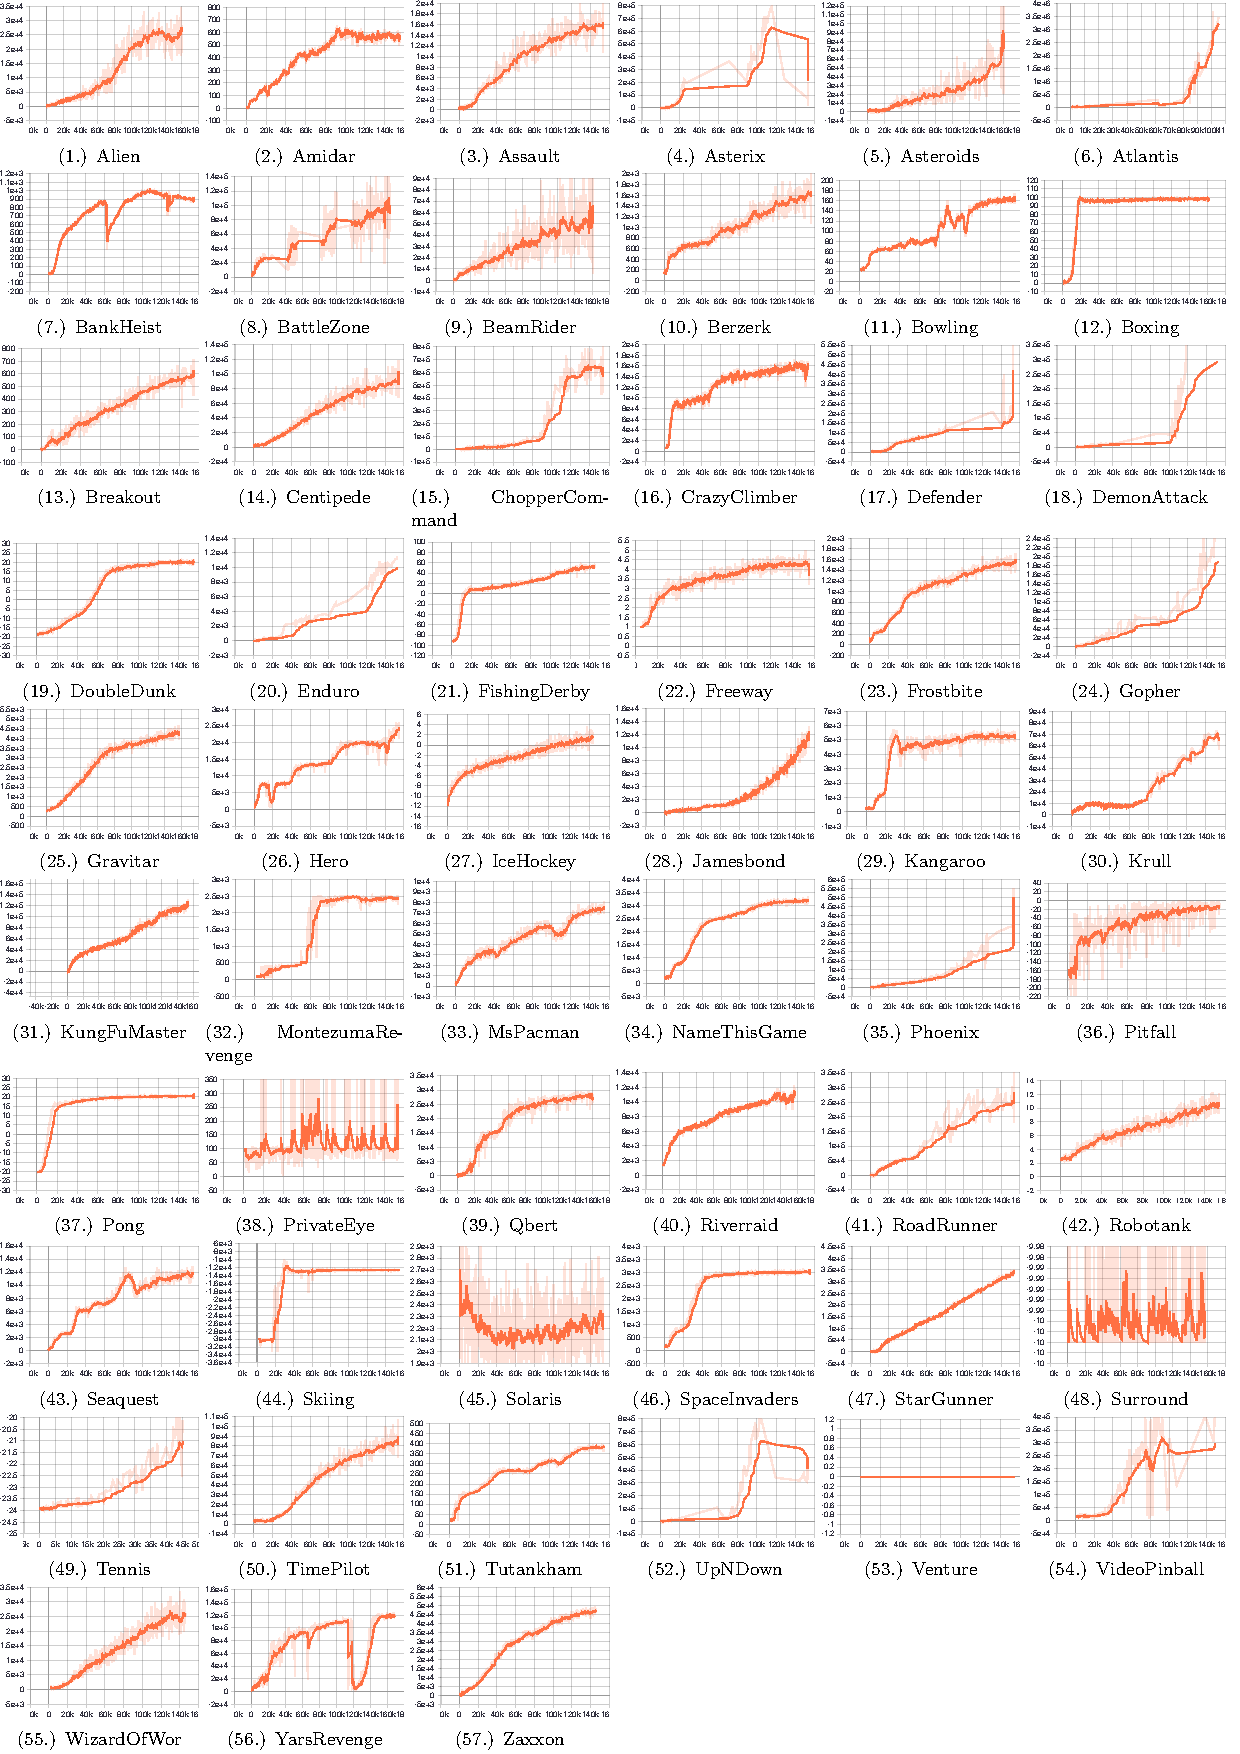
\includegraphics[width=1.0\linewidth]{body/all_fig3.pdf}
\end{figure*}

\clearpage



\end{document}